\documentclass[conference]{IEEEtran}
\IEEEoverridecommandlockouts
\usepackage[a-1b]{pdfx}
\usepackage{balance}
\usepackage{hyperref} 
\usepackage{booktabs} 
\usepackage{xcolor}    
\usepackage{colortbl} 
\usepackage{subcaption}
\captionsetup[figure]{name={Figure},labelsep=period, font=footnotesize}
\captionsetup[table]{labelsep=period, font={sc,footnotesize} }


\usepackage{cite}
\usepackage{amsmath,amssymb,amsfonts}
\usepackage{algorithmic}
\usepackage{graphicx}
\usepackage{textcomp}
% \usepackage{xcolor}
\def\BibTeX{{\rm B\kern-.05em{\sc i\kern-.025em b}\kern-.08em
    T\kern-.1667em\lower.7ex\hbox{E}\kern-.125emX}}
\begin{document}


\title{Pre‑Tactical Flight‑Delay and Turnaround Forecasting with Synthetic Aviation Data}



\author{
    \IEEEauthorblockN{Abdulmajid Murad$^{1}$, Massimiliano Ruocco$^{1,2}$}
    \IEEEauthorblockA{
        \parbox{0.5\textwidth}{
            \centering
            $^1$Department of Software Engineering, Safety and Security \\ 
            SINTEF Digital \\
            Trondheim, Norway \\
            \{abdulmajid.murad, massimiliano.ruocco\}@sintef.no
        }
        \hspace{0.05\textwidth}
        \parbox{0.4\textwidth}{
            \centering
            $^2$Department of Computer Science \\
            Norwegian University of Science and Technology \\
            Trondheim, Norway \\
            massimiliano.ruocco@ntnu.no
        }
    }
}


\maketitle



\begin{abstract}

    Access to comprehensive flight operations data remains severely restricted in aviation due to commercial sensitivity and competitive considerations, hindering the development of predictive models for operational planning. This paper investigates whether synthetic data can effectively replace real operational data for training machine learning models in pre-tactical aviation scenarios—predictions made hours to days before operations using only scheduled flight information. We evaluate four state-of-the-art synthetic data generators on three prediction tasks: aircraft turnaround time, departure delays, and arrival delays. Using a Train on Synthetic, Test on Real (TSTR) methodology on over 1.7 million European flight records, we assess both predictive performance and the preservation of operational relationships. Our results show that transformer-based synthetic data generators can retain 94-97\% of real-data predictive performance while maintaining feature importance patterns informative for operational decision-making. We also quantify fundamental predictability limits in pre-tactical scenarios, highlighting inherent operational uncertainties. These findings suggest that high-quality synthetic data can enable broader access to aviation analytics capabilities while preserving commercial confidentiality, though stakeholders must maintain realistic expectations about pre-tactical prediction accuracy given the stochastic nature of flight operations.


\end{abstract}

\begin{IEEEkeywords}
Synthetic Data, Air Traffic Management (ATM), Flight Delay Prediction, Turnaround Time, Machine Learning, Data Utility, Generative Models, Aviation Operations
\end{IEEEkeywords}

\section{Introduction}


The aviation industry generates substantial operational data that could be valuable for optimizing flight operations, improving resource allocation, and enhancing passenger experience. However, access to this data is often restricted due to commercial sensitivity, privacy regulations, and competitive considerations. Airlines typically guard their operational data as commercially sensitive and proprietary, concerned that disclosure could affect their competitive strategies.%\cite{majumder2025dgca}. 
Additionally, data protection laws such as GDPR and security concerns create tensions between data openness and privacy protection \cite{lei2025fedmeta}. This limited access affects external researchers, smaller airlines, and emerging markets that lack the historical datasets needed for developing predictive analytics.


The challenge of data scarcity is particularly relevant in pre-tactical flight operations—the period hours to days before actual flights when airlines, airports, and passengers must make decisions based on anticipated conditions. Unlike tactical predictions made on the day of operations with real-time updates, pre-tactical models must rely primarily on published schedules and historical patterns \cite{dalmau2024probabilistic}. While tactical models can incorporate live weather updates, air traffic flow restrictions, and current aircraft positions, pre-tactical predictions operate with more limited information where only scheduled characteristics and statistical patterns are available \cite{mas2022pre}.

Despite these information constraints, pre-tactical predictions can provide value across the aviation ecosystem. Airlines use these forecasts to adjust operations—modifying aircraft assignments, crew schedules, or flight times before disruptions propagate through their networks \cite{mas2022pre}. Airports utilize predictions to plan gate requirements and staffing needs based on expected delays and turnaround times \cite{de2023probabilistic}. For passengers, advance notice of potential delays can inform decisions about connections and travel arrangements \cite{carvalho2021relevance}. However, organizations with limited access to historical data—including smaller airlines, regional airports, and academic researchers—face challenges in developing these predictive capabilities.


The uncertainty in pre-tactical prediction stems from various factors that influence actual operations but remain unknown at schedule publication time. Weather conditions, air traffic congestion, technical issues, crew availability, airport capacity constraints, and cascading delays from earlier flights all contribute to deviations from scheduled operations \cite{carvalho2021relevance}. For aircraft turnaround time—the period between arrival and subsequent departure—predictions must account for ground processes including passenger handling, cleaning, catering, fueling, and maintenance, each varying by aircraft type, airport infrastructure, and time of day \cite{de2023probabilistic}. Similarly, departure and arrival delay predictions must infer potential disruptions based on historical patterns and scheduled characteristics, without access to current operational status.

This operational complexity presents two related challenges. First, even with comprehensive data access, pre-tactical predictions face accuracy limitations due to the stochastic nature of aviation operations \cite{dalmau2024probabilistic}. Weather patterns, technical failures, and human factors introduce uncertainties that are difficult to capture days in advance. Second, the restricted availability of operational data prevents many organizations from developing baseline predictive models. Without historical records showing how scheduled operations translated into actual performance under various conditions, stakeholders cannot build fundamental predictive capabilities.



Recent work in synthetic data generation presents one approach to addressing data availability while respecting commercial confidentiality. By creating artificial datasets that preserve statistical properties and predictive relationships of real operations without exposing sensitive information, synthetic data could enable broader access to analytics capabilities. The Train on Synthetic, Test on Real (TSTR) paradigm \cite{esteban2017real} suggests that models trained on synthetic data can generalize to real-world scenarios, potentially allowing organizations without historical data access to develop operational prediction capabilities. Recent work has shown that synthetic flight data can approximate real data's statistical profiles, with models trained on synthetic data achieving prediction accuracies comparable to those trained on actual data \cite{aly2025synthetic}.


However, the effectiveness of synthetic data for pre-tactical aviation prediction requires further investigation. The challenges of pre-tactical scenarios—where predictive relationships are embedded in complex interactions between limited scheduled features—require evaluation beyond traditional distributional similarity metrics. An important consideration is whether synthetic data can preserve not only the statistical properties of flight operations but also the latent patterns that enable prediction of future delays and extended turnarounds from scheduled information.


This study evaluates the utility of synthetic flight data across three pre-tactical prediction tasks: aircraft turnaround time, departure delays, and arrival delays. We assess four synthetic data generation approaches—Gaussian Copula (statistical modeling), Conditional Tabular GAN (adversarial learning) \cite{xu2019modeling}, TabSyn (diffusion-based synthesis) \cite{zhang2024mixed}, and REaLTabFormer (transformer architecture) \cite{solatorio2023realtabformer}—examining their effectiveness in preserving relationships necessary for operational forecasting when only scheduled information is available.



Our evaluation examines both predictive performance and the preservation of feature relationships, aiming to ensure that models trained on synthetic data achieve acceptable accuracy while identifying relevant operational drivers. This is important for practical deployment, where understanding prediction rationale can be as valuable as the predictions themselves.



Using over 1.7 million European flight records, our analysis contributes:
\begin{itemize}
\item An evaluation framework for assessing synthetic data utility in pre-tactical aviation contexts, accounting for limited feature availability and operational uncertainty.
\item Quantitative analysis of performance differences when substituting synthetic for real training data across multiple operational prediction tasks, finding that transformer-based methods can retain 94-97\% of real-data predictive performance.
\item Identification of synthetic generation approaches that preserve predictive relationships when operational information is limited, with REaLTabFormer demonstrating consistent performance in maintaining feature importance patterns.
\item An open-source implementation of the used generative models and evaluation pipeline, making the methods accessible for further research and benchmarking.\footnote{Code available at: \href{https://github.com/SynthAIr/syntabair}{https://github.com/SynthAIr/syntabair}}
% \item Baseline expectations for predictability limits in pre-tactical scenarios, showing that even with real data, R² values typically remain below 0.44, providing context for operational planning regardless of data source.
\end{itemize}


Through this analysis, we explore whether synthetic data can serve as a practical substitute for proprietary operational records in pre-tactical prediction tasks. Our findings suggest potential pathways for broader access to analytics capabilities across the industry while maintaining commercial confidentiality requirements.

\section{Related Work}

The challenge of predicting flight delays and turnaround times has attracted significant attention in recent years. De Falco et al. \cite{de2023probabilistic} developed probabilistic machine learning models to forecast aircraft turnaround times and Target Off-Block Times (TOBT) at major European airports. This work uniquely focused on turnaround operations, which are critical contributors to reactionary delays, and provided probabilistic outputs rather than point estimates.

In the domain of delay prediction, Mas-Pujol et al. \cite{mas2022pre} presented a machine learning framework to predict individual flight delays. Their model employs a two-stage approach: first classifying whether flights will experience delays and identifying the cause category, then predicting delay duration. The study identified crucial features including flight timing, airport demand, and weather conditions that influence pre-tactical delays, demonstrating the advantages of data-driven approaches over traditional simulation methods.

Dalmau et al. \cite{dalmau2024probabilistic} introduced probabilistic delay prediction using quantile regression. Their work predicts delay distributions rather than single estimates, enabling better uncertainty quantification. Notably, their analysis revealed that expected passenger numbers significantly influenced delay predictions - an insight often unavailable in other studies due to data limitations.

A comprehensive survey by Wandelt et al. \cite{wandelt2025flight}  examined approximately 40 recent flight delay prediction studies. Their analysis revealed that machine learning approaches, particularly random forests and neural networks, have become dominant in capturing delay factors. Common features across studies include scheduled information, weather conditions, and route characteristics, highlighting the consistent importance of weather and operational timing in delay forecasting.

The proprietary nature of aviation datasets has driven researchers toward synthetic data generation as an alternative approach. Most existing work has concentrated on trajectory data generation. Krauth et al. \cite{krauth2023deep}, Ezzahed et al. \cite{ezzahed2022bringing}, and Krauth et al. \cite{krauth2024advanced} demonstrated the effectiveness of Variational Autoencoders (VAEs) for modeling aircraft trajectories in terminal maneuvering areas. Wijnands et al. \cite{wijnands2024generation} explored Generative Adversarial Networks (GANs), specifically the TimeGAN framework, for creating synthetic landing trajectories. Murad and Ruocco \cite{murad2025synthetic} extended this trajectory-focused work by applying vector-quantized VAEs to generate synthetic flight paths between airport pairs. Their results showed that synthetic trajectories could effectively capture the statistical properties of real flight data, though these approaches remain limited to spatial trajectory modeling rather than operational records. 

A notable departure from trajectory-focused work comes from Aly and Sharpanskykh \cite{aly2025synthetic}, who broadened synthetic data generation to encompass flight operational records. Their study generated tabular datasets including flight schedules, aircraft information, and delay data. However, their evaluation was limited to two generative models (TVAE and Gaussian Copula) and used publicly available U.S. domestic flight data.


While substantial progress has been made in both flight delay prediction and synthetic data generation, a critical gap remains in combining these approaches for pre-tactical operational planning. Existing delay prediction models rely on access to comprehensive historical datasets, which many smaller operators and researchers lack. Similarly, synthetic data generation in aviation has primarily focused on trajectories rather than the operational records needed for delay prediction. This work addresses this gap by investigating whether synthetic operational data can enable effective pre-tactical delay prediction without requiring access to sensitive historical records.



\section{Methodology}

Our methodology, illustrated in Figure \ref{fig:framework}, is structured into four sequential phases: Data Preparation, Synthetic Generation, Model Training, and Evaluation. First, we process the raw flight data, selecting only pre-tactical features and splitting the dataset into training and testing sets. Second, the real training data is used to train four different synthetic data generators. Third, we establish two parallel training pipelines: a baseline where predictive models are trained on the real training data (TRTR), and an evaluation pipeline where the same models are trained on the generated synthetic data (TSTR). Finally, we evaluate all trained models on the held-out real test set, comparing their performance on three prediction tasks to assess the utility of the synthetic data.

\begin{figure*}[t]
    \centering
    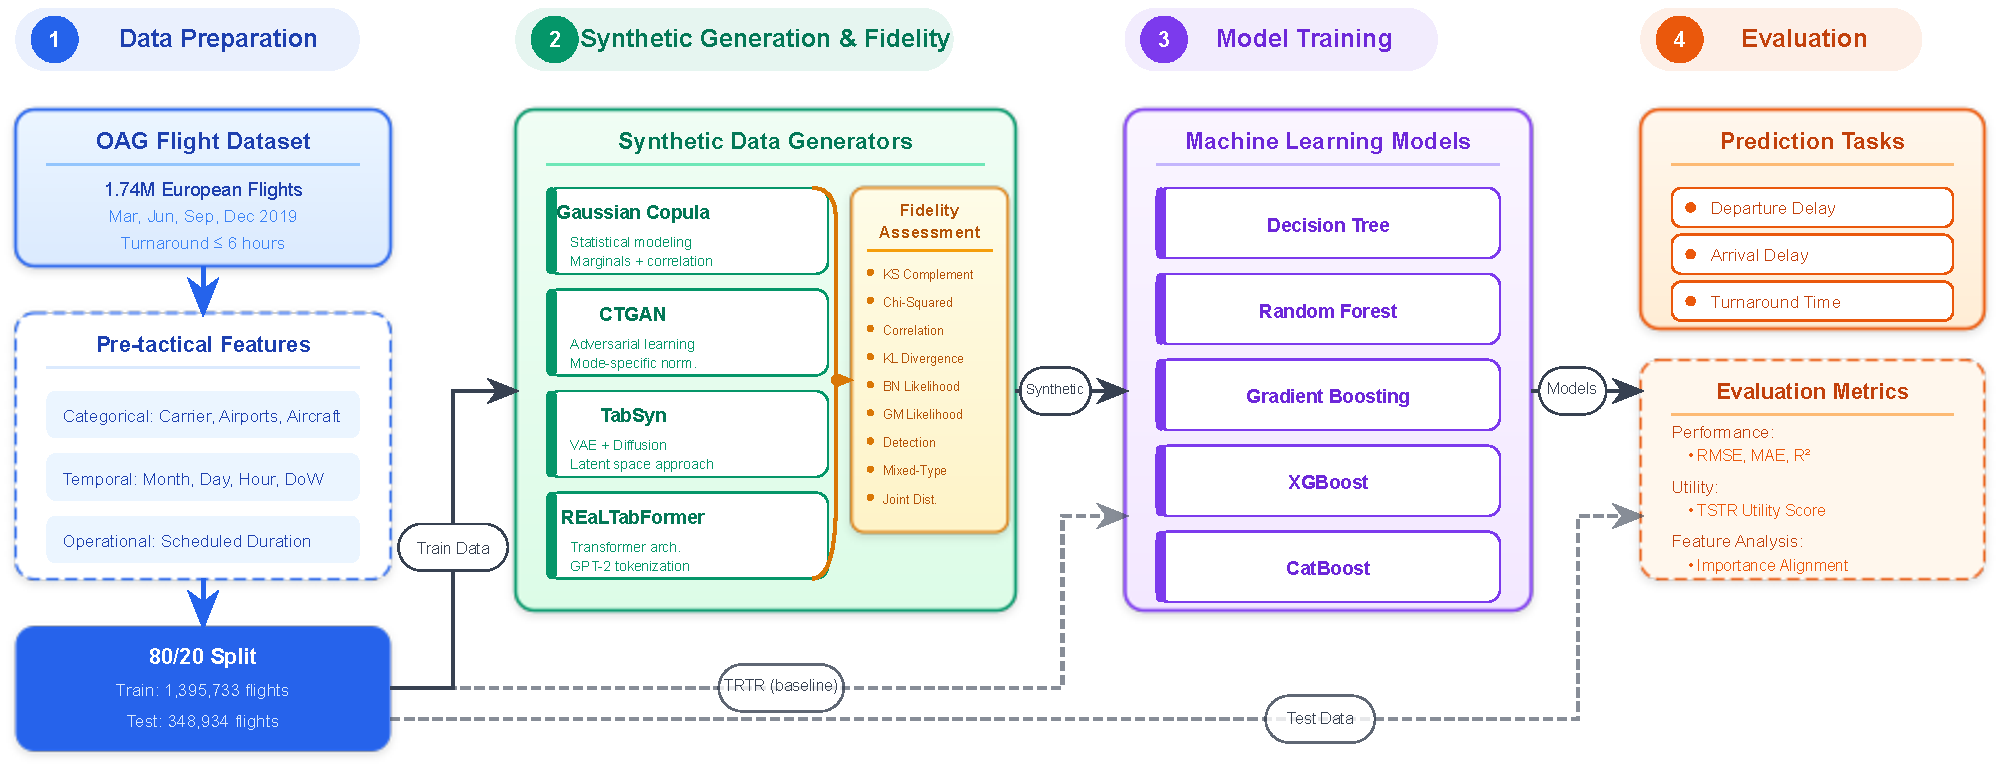
\includegraphics[width=\textwidth]{diagrams/overall_framework.pdf}
    \caption{The experimental framework, illustrating the four main phases. 1) Real-world flight data is prepared and split. 2) The real training data is used to train four types of synthetic data generators. 3) Five machine learning models are trained in two settings: on the real training data (TRTR baseline) and on each of the synthetic datasets (TSTR). 4) All models are evaluated on the unseen real test data across three prediction tasks using performance, utility, and feature alignment metrics.}
    \label{fig:framework}
\end{figure*}

\subsection{Dataset}

We utilized OAG's Flight Info Direct Status Summary database\footnote{'Status Direct: Data Fields Explained'. Accessed: June 17, 2025. [Online]. Available: \url{https://knowledge.oag.com/docs/status-direct-data-fields-explained}}, extracting European flight operations from March, June, September, and December 2019. After filtering for completed flights with full operational timelines and valid turnaround observations, we obtained 1,744,667 flight records.

\subsubsection{Feature Selection}
For pre-tactical prediction, we selected only features available at schedule publication time:

\textbf{Categorical}: IATA carrier code, departure/arrival airports, aircraft type

\textbf{Temporal}: Month, day, hour, minute (extracted from scheduled departure), day of week

\textbf{Operational}: Scheduled flight duration (actual duration excluded in pre-tactical mode)

\subsubsection{Target Variables}
We computed three operational metrics:
\begin{itemize}
    \item \textbf{Departure delay}: $\Delta_{\text{dep}} = t_{\text{AOBT}} - t_{\text{SOBT}}$ (Actual vs. Scheduled Off-Block Time)
    \item \textbf{Arrival delay}: $\Delta_{\text{arr}} = t_{\text{AIBT}} - t_{\text{SIBT}}$ (Actual vs. Scheduled In-Block Time)
    \item \textbf{Turnaround time}: Ground time between consecutive flights of the same aircraft at the same airport, constrained to $\leq$ 6 hours to exclude overnight parking
\end{itemize}

The turnaround matching process ensured all records have valid turnaround observations, enabling consistent evaluation across all three prediction tasks. The dataset exhibits mean departure delay of 11.1 minutes ($\sigma$=24.0), mean arrival delay of 7.5 minutes ($\sigma$=25.8), and mean turnaround time of 70.8 minutes ($\sigma$=51.2).

We applied an 80/20 train-test split (1,395,733/348,934 flights) with fixed random seed for reproducibility.


\subsection{Synthetic Data Generation}
Four state-of-the-art synthetic data generators were evaluated, each representing different technical approaches to capturing the complex relationships in flight data:

\subsubsection{Gaussian Copula (GC)}
A statistical approach that models multivariate dependencies by separating marginal distributions from their dependence structure. This method is particularly suited for mixed-type tabular data, handling both categorical (airports, carriers, aircraft types) and continuous (delays, turnaround times) variables through a unified framework.

The Gaussian copula model operates in two stages:

\textbf{Marginal Distribution Fitting:} For each variable $X_i$ in the dataset, we fit an appropriate univariate distribution. For continuous variables, the implementation employs a flexible selection mechanism that evaluates multiple candidate distributions (e.g., Gaussian, exponential, beta) using the Kolmogorov-Smirnov test, automatically selecting the best-fitting model. Categorical variables are encoded using ordinal encoding, preserving their discrete nature while enabling numerical processing.

\textbf{Dependency Modeling:} After fitting marginals, we transform each variable to the standard normal domain using:
\begin{equation}
Z_i = \Phi^{-1}(F_i(X_i))
\end{equation}
where $F_i$ is the fitted CDF for variable $i$ and $\Phi^{-1}$ is the inverse standard normal CDF. The transformation clips extreme values to $[\epsilon, 1-\epsilon]$ to ensure numerical stability.

The correlation structure is then captured by computing the correlation matrix $\mathbf{R}$ of the transformed variables $\{Z_1, ..., Z_d\}$. For random variables $X_1, X_2, \ldots, X_d$ with marginal CDFs $F_1, F_2, \ldots, F_d$, let $u_i = F_i(X_i)$ represent the probability integral transforms. The joint distribution is then modeled using the Gaussian copula:
\begin{equation}
C_{\mathbf{R}}(u_1, ..., u_d) = \Phi_{\mathbf{R}}(\Phi^{-1}(u_1), ..., \Phi^{-1}(u_d))
\end{equation}
where $\Phi_{\mathbf{R}}$ represents the CDF of a multivariate normal distribution with correlation matrix $\mathbf{R}$.


\textbf{Synthetic Data Generation:} To generate new samples:
\begin{enumerate}
    \item Sample $\mathbf{z} \sim \mathcal{N}(\mathbf{0}, \mathbf{R})$ from the multivariate normal
    \item Transform to uniform: $u_i = \Phi(z_i)$ for each component
    \item Apply inverse marginal CDFs: $x_i = F_i^{-1}(u_i)$
    \item For categorical variables, round to nearest valid category index and decode
\end{enumerate}

This approach preserves parametrically-fitted marginal distributions while capturing linear correlations between variables. However, it may struggle with complex non-linear dependencies and rare event combinations that are particularly important in aviation operations.


\subsubsection{Conditional Tabular GAN (CTGAN)} \cite{xu2019modeling}
A generative adversarial network specifically designed for mixed-type tabular data. Key innovations include:
\begin{itemize}
    \item \textbf{Mode-specific normalization}: Uses Bayesian Gaussian Mixture Models to handle multimodal continuous distributions
    \item \textbf{Conditional generation}: Employs training-by-sampling with log-frequency to address category imbalance
    \item \textbf{PacGAN framework}: Prevents mode collapse by having the discriminator evaluate multiple samples jointly
    \item \textbf{WGAN-GP loss}: Ensures training stability through gradient penalty regularization
\end{itemize}

\subsubsection{TabSyn} \cite{zhang2024mixed}
A two-stage approach combining Variational Autoencoders (VAE) with diffusion models:
\begin{enumerate}
    \item \textbf{Stage 1 - VAE Training}: Learns continuous latent representations of mixed-type data using:
    \begin{equation}
    \mathcal{L}_{\text{VAE}} = \mathcal{L}_{\text{recon}} + \beta \cdot \mathcal{L}_{\text{KL}}
    \end{equation}
    where $\beta$ is adaptively scheduled during training
    \item \textbf{Stage 2 - Diffusion in Latent Space}: Applies score-based diffusion to generate new latent vectors, requiring only 20-50 reverse steps compared to thousands in traditional diffusion
\end{enumerate}

\subsubsection{REaLTabFormer} \cite{solatorio2023realtabformer}
A transformer-based model that treats each table row as a sequence of tokens. The architecture leverages:
\begin{itemize}
    \item \textbf{GPT-2 backbone}: 6 decoder layers with 768-dimensional embeddings
    \item \textbf{Column-aware tokenization}: Separate vocabularies for each column type
    \item \textbf{Regularization mechanisms}: Random masking (10\%) and bootstrap-based $Q_\delta$ testing to prevent memorization
    \item \textbf{Constrained sampling}: Domain-specific token filtering during generation
\end{itemize}

\subsection{Pre-tactical Prediction Tasks}

We evaluated three operational prediction scenarios, all in pre-tactical mode where only scheduled information is available:

\subsubsection{Turnaround Time Prediction}
Forecasting the duration between aircraft arrival (In-Block) and departure (Off-Block) using:
\begin{itemize}
    \item Input features: Scheduled times, airports, carrier, aircraft type, temporal features
    \item Target: Actual turnaround time in minutes
    \item Operational relevance: Critical for gate allocation and ground resource planning
\end{itemize}

\subsubsection{Departure Delay Prediction}
Estimating the difference between scheduled and actual departure times:
\begin{itemize}
    \item Input features: Same as turnaround prediction
    \item Target: Departure delay in minutes (positive for late departures)
    \item Operational relevance: Enables proactive delay mitigation strategies
\end{itemize}

\subsubsection{Arrival Delay Prediction}
Forecasting arrival delays using only pre-departure information:
\begin{itemize}
    \item Input features: Same as above predictions
    \item Target: Arrival delay in minutes
    \item Challenge: Most difficult task due to cumulative uncertainties from departure delays and en-route factors
\end{itemize}

\subsection{Evaluation Framework}

Our evaluation employed multiple complementary metrics to assess synthetic data quality comprehensively:

\subsubsection{Predictive Performance Metrics}
\begin{itemize}
    \item \textbf{Root Mean Squared Error (RMSE)}: Emphasizes large prediction errors critical for disruption management:
    \begin{equation}
    \text{RMSE} = \sqrt{\frac{1}{n}\sum_{i=1}^{n}(y_i - \hat{y}_i)^2}
    \end{equation}
    
    \item \textbf{Mean Absolute Error (MAE)}: Provides typical error magnitude for operational planning:
    \begin{equation}
    \text{MAE} = \frac{1}{n}\sum_{i=1}^{n}|y_i - \hat{y}_i|
    \end{equation}
    
    \item \textbf{Coefficient of Determination (R²)}: Measures explained variance to assess predictability limits:
    \begin{equation}
    R^2 = 1 - \frac{\sum_{i=1}^{n}(y_i - \hat{y}_i)^2}{\sum_{i=1}^{n}(y_i - \bar{y})^2}
    \end{equation}
\end{itemize}

\subsubsection{Utility Score}
A normalized metric combining RMSE and R² performance to quantify how well synthetic-trained models substitute for real-trained models:

\begin{equation}
\text{Utility} = 0.5 \times \min\left(\frac{\text{RMSE}_{\text{real}}}{\text{RMSE}_{\text{synthetic}}}, 1.0\right) + 0.5 \times \min\left(\frac{R^2_{\text{synthetic}}}{R^2_{\text{real}}}, 1.0\right)
\end{equation}

\subsubsection{Feature Importance Alignment}
To ensure synthetic data preserves operational relationships, we compute the cosine similarity between feature importance vectors from models trained on real ($\mathbf{v}_{\text{real}}$) versus synthetic ($\mathbf{v}_{\text{synthetic}}$) data:

\begin{equation}
\text{Alignment} = \frac{\mathbf{v}_{\text{real}} \cdot \mathbf{v}_{\text{synthetic}}}{||\mathbf{v}_{\text{real}}|| \cdot ||\mathbf{v}_{\text{synthetic}}||}
\end{equation}

\subsection{Machine Learning Pipeline}

\subsubsection{Model Selection}
We employed five regression algorithms to ensure robust evaluation across different modeling paradigms:
\begin{itemize}
    \item \textbf{Decision Tree}: Captures non-linear patterns through recursive partitioning
    \item \textbf{Random Forest}: Ensemble of trees for improved generalization
    \item \textbf{Gradient Boosting}: Sequential ensemble focusing on residual errors
    \item \textbf{XGBoost}: Optimized gradient boosting with regularization
    \item \textbf{CatBoost}: Gradient boosting specialized for categorical features
\end{itemize}

\subsubsection{Training Protocol}
\begin{enumerate}
    \item \textbf{Train on Real, Test on Real (TRTR)}: Baseline performance using historical data
    \item \textbf{Train on Synthetic, Test on Real (TSTR)}: Utility evaluation of synthetic data
    \item \textbf{Feature Engineering}: All models used identical pre-tactical features to ensure fair comparison
    \item \textbf{Hyperparameter Optimization}: Default parameters were used to avoid biasing results toward specific generators
\end{enumerate}


\section{Results and Discussion}

\subsection{Departure Delay Prediction}

Pre-tactical departure delay prediction emerged as one of the most challenging tasks, with real-data models achieving R² values between 0.10 and 0.30 (Figure~\ref{fig:departure_r2}). This limited predictability reflects the numerous external factors influencing departure times—weather conditions, air traffic flow restrictions, crew availability, and technical issues—that are not captured in scheduled information alone. The inherent stochasticity of these factors creates a fundamental ceiling on pre-tactical prediction accuracy, regardless of data quality.

\begin{figure}[htbp]
    \centering
    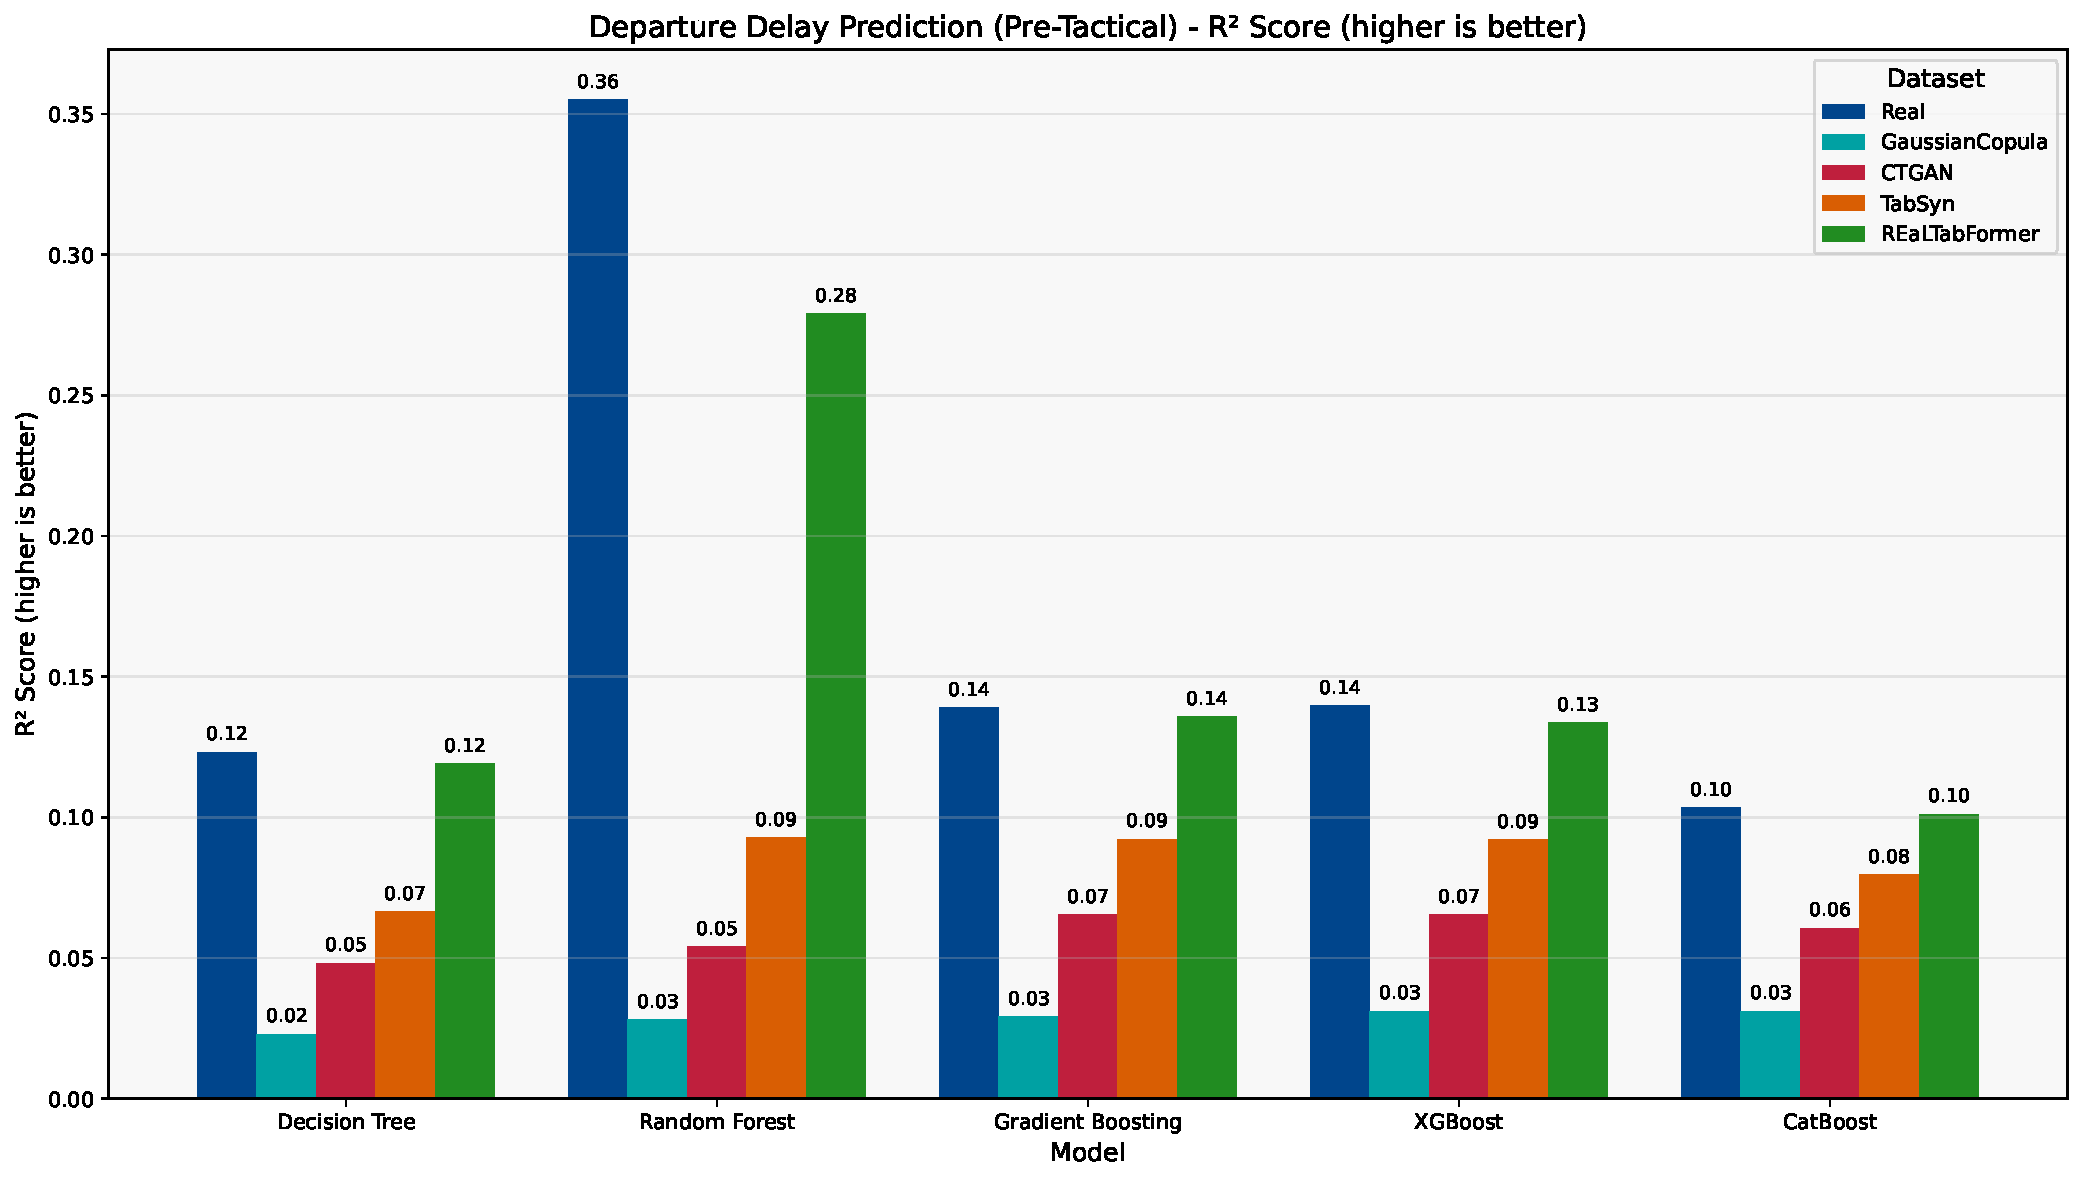
\includegraphics[width=\linewidth]{plots/departure_delay_min_pre-tactical/departure_delay_min_pre-tactical_r2.pdf}
    \caption{Coefficient of determination (R²) for pre-tactical departure delay prediction across different models and synthetic data generators.}
    \label{fig:departure_r2}
\end{figure}

Despite these constraints, clear performance hierarchies emerged among synthetic generators. The RMSE and MAE metrics reveal REaLTabFormer's superiority in preserving the subtle predictive patterns present in scheduled data (Figures~\ref{fig:departure_pre_rmse} and \ref{fig:departure_pre_mae}). REaLTabFormer consistently achieved the lowest error rates, with RMSE values within 4\% of real-data baselines. The transformer architecture's ability to capture long-range dependencies between categorical features (airlines, airports) and temporal patterns proves crucial for this task.

\begin{figure}[htbp]
    \centering
    \begin{subfigure}[b]{0.49\textwidth}
        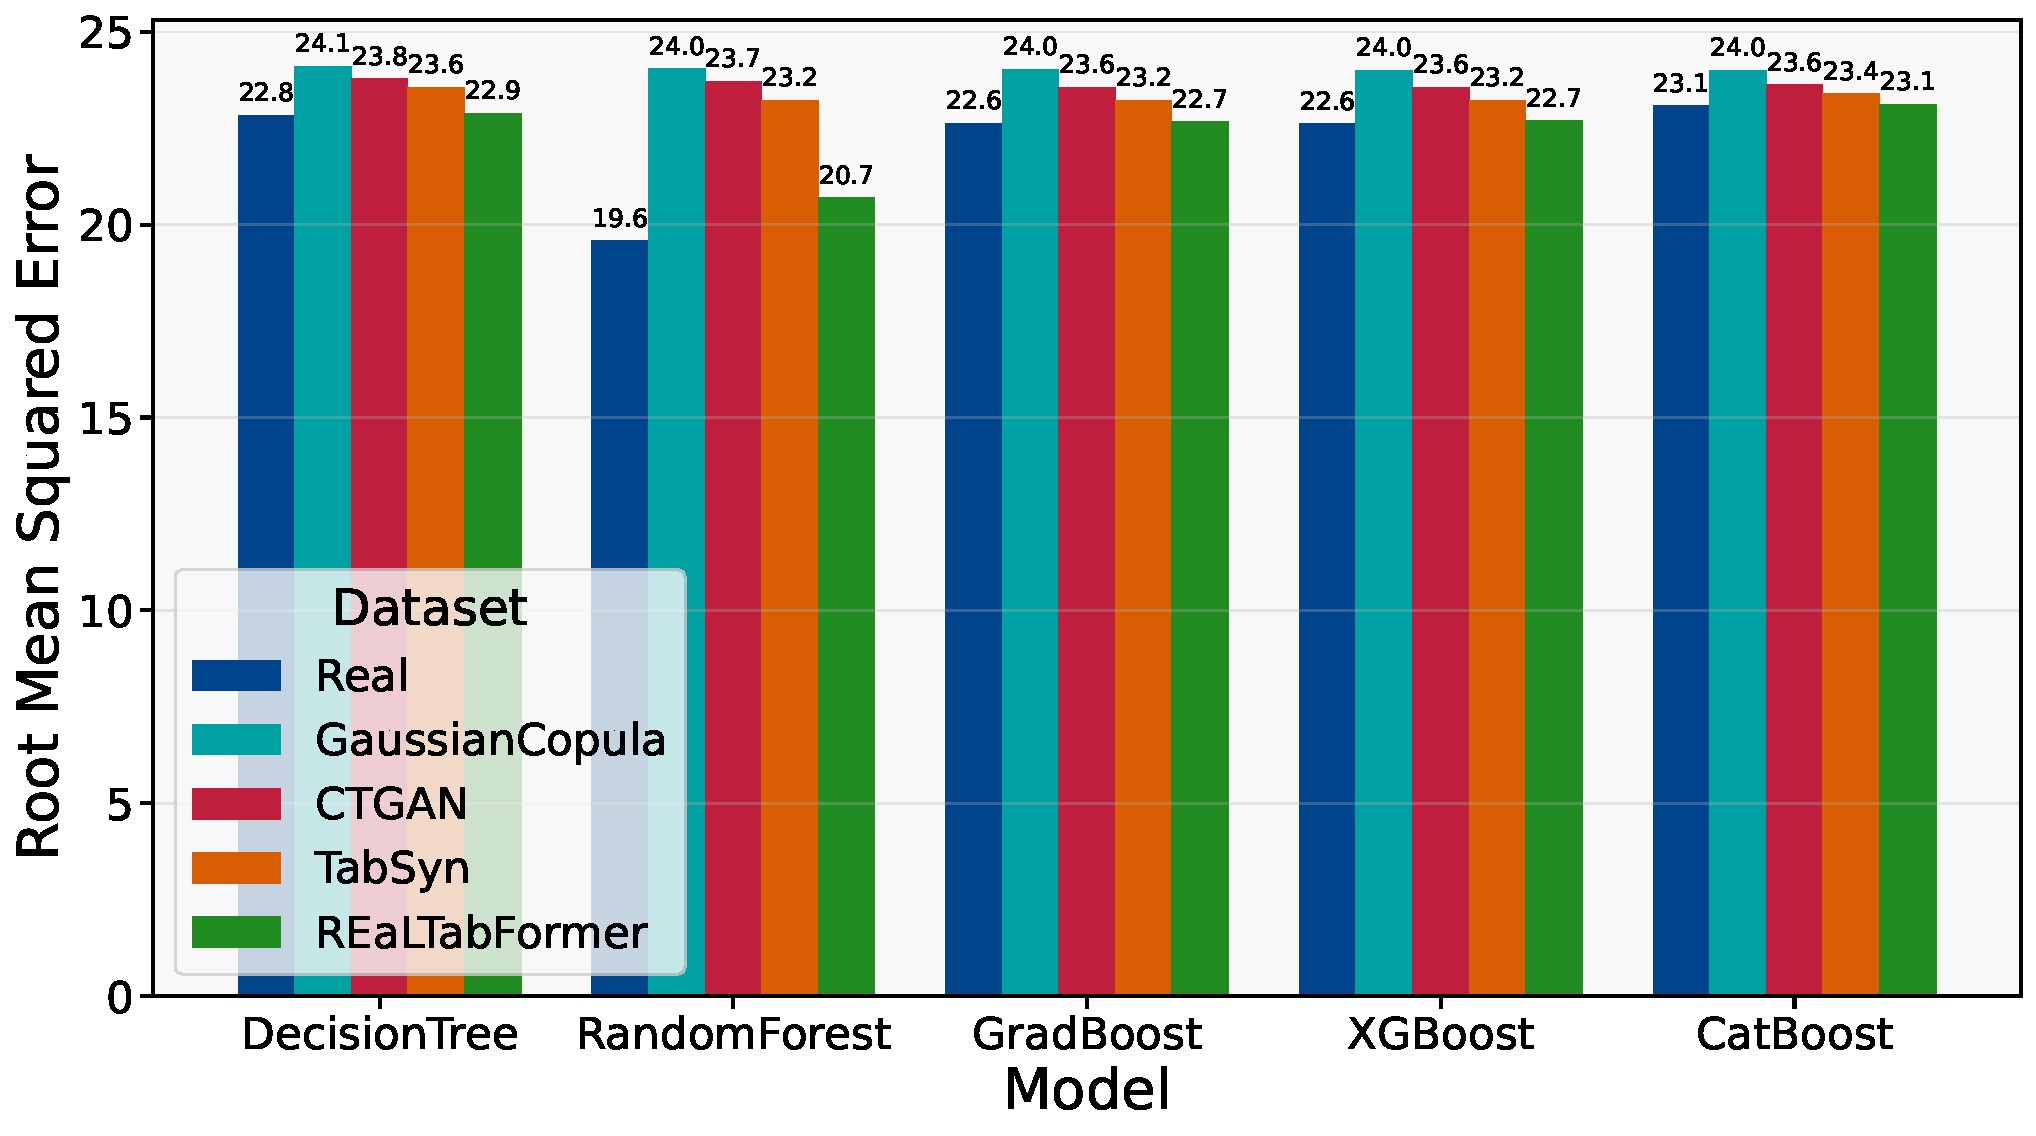
\includegraphics[width=\linewidth]{plots/departure_delay_min_pre-tactical/departure_delay_min_pre-tactical_rmse.pdf}
        \caption{Root Mean Squared Error}
        \label{fig:departure_pre_rmse}
    \end{subfigure}
    \hfill
    \begin{subfigure}[b]{0.49\textwidth}
        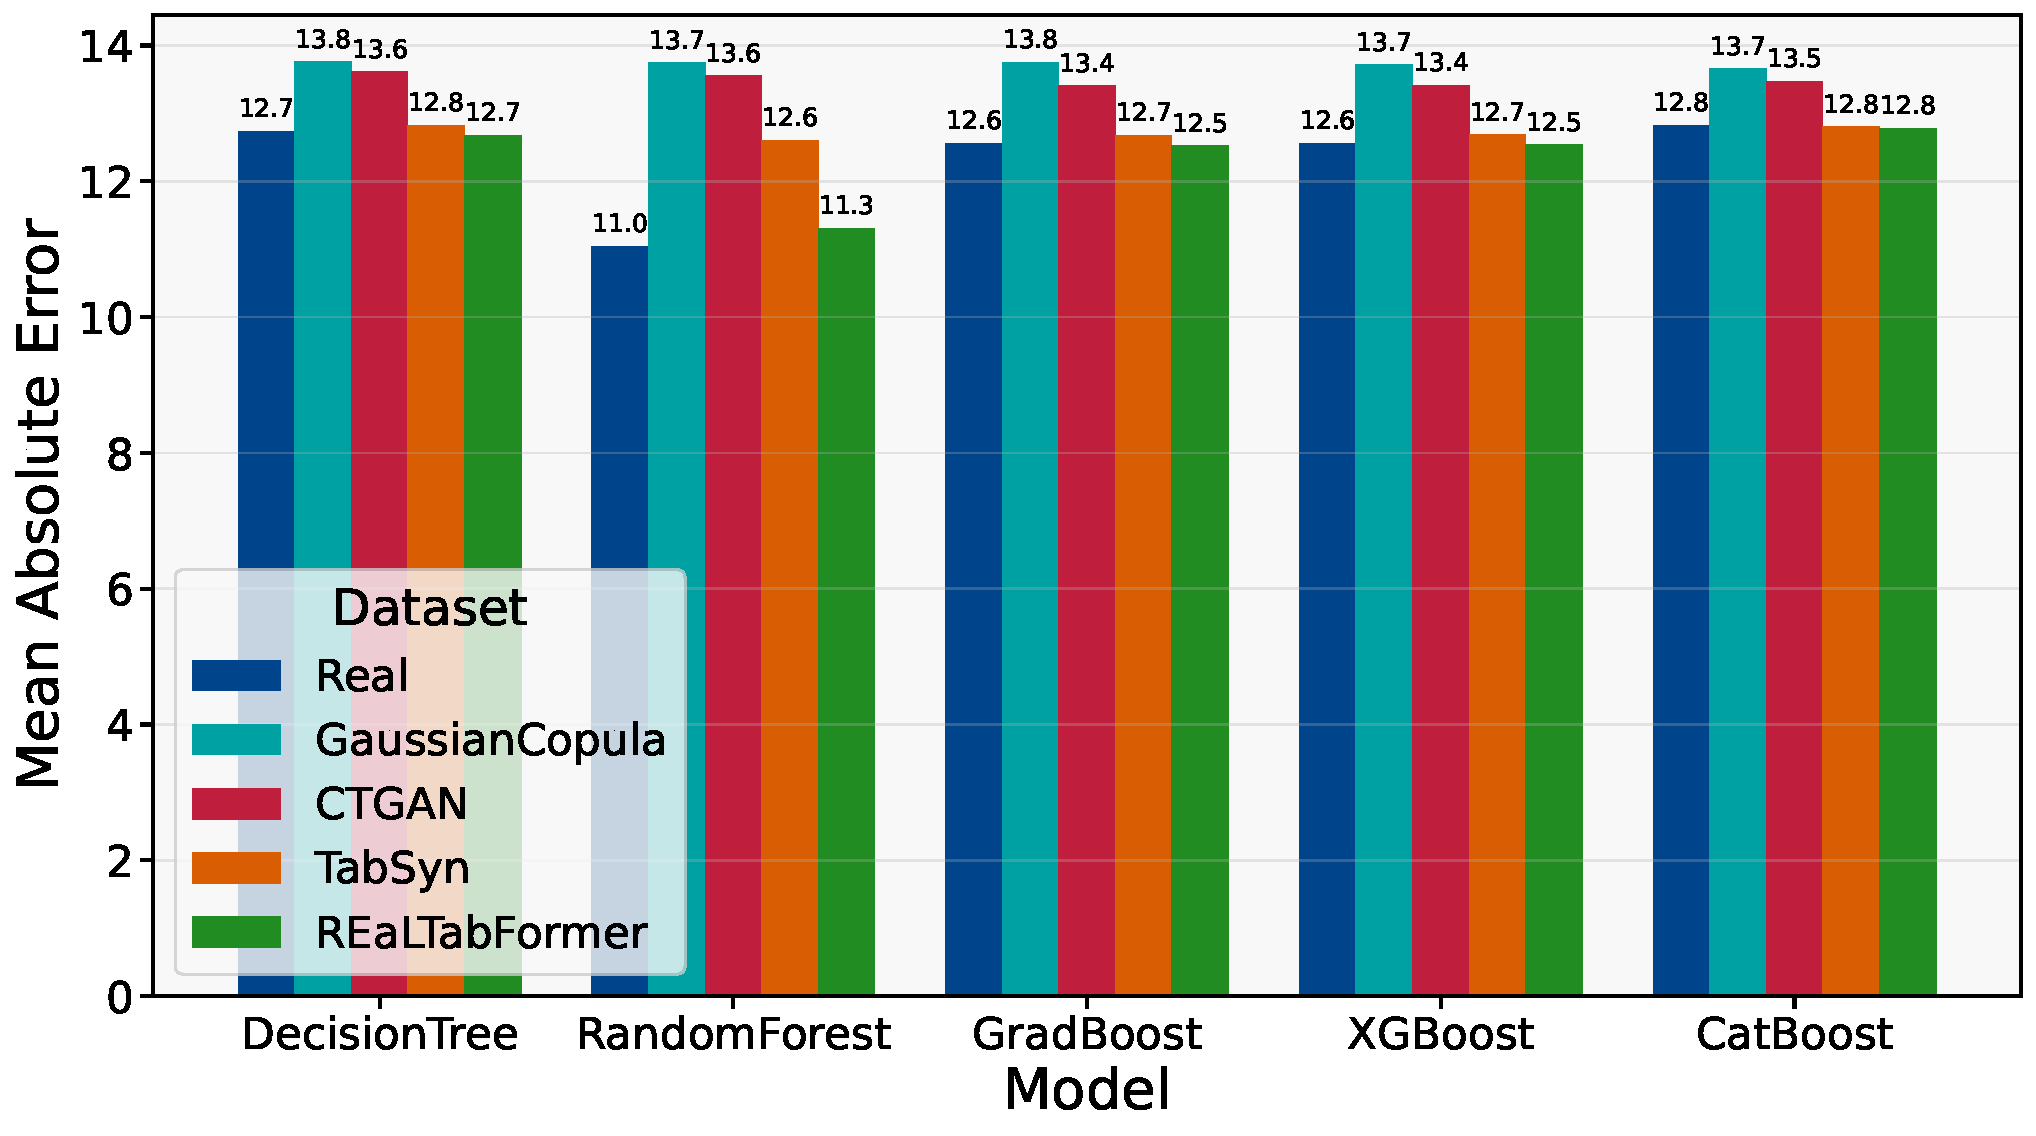
\includegraphics[width=\linewidth]{plots/departure_delay_min_pre-tactical/departure_delay_min_pre-tactical_mae.pdf}
        \caption{Mean Absolute Error}
        \label{fig:departure_pre_mae}
    \end{subfigure}
    \caption{Prediction error metrics for pre-tactical departure delay across models and synthetic data generators.}
\end{figure}

The utility scores quantify the practical impact of these differences (Figure~\ref{fig:departure_utility}). REaLTabFormer achieved a utility score of 0.96, indicating that models trained on its synthetic data retain 96\% of the predictive capability of models trained on real data. This represents a remarkable preservation of predictive relationships given the task's inherent difficulty. TabSyn's utility dropped more significantly to 0.76, suggesting that departure delay patterns require sophisticated modeling of rare events and edge cases that simpler diffusion approaches struggle to capture consistently.

\begin{figure}[htbp]
    \centering
    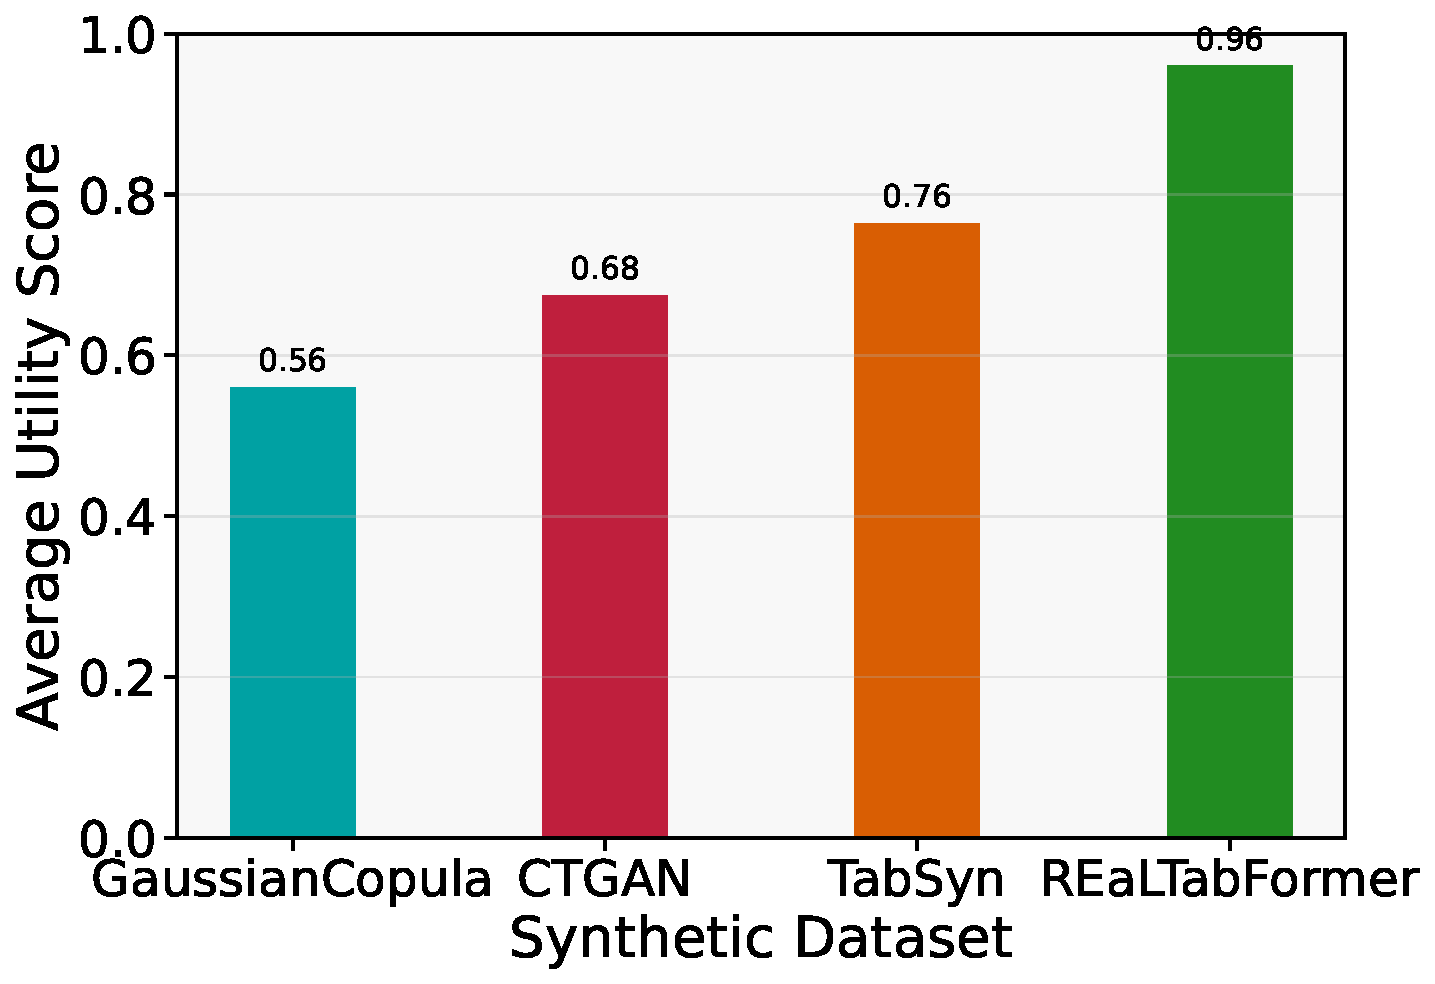
\includegraphics[width=0.8\linewidth]{plots/departure_delay_min_pre-tactical/departure_delay_min_pre-tactical_avg_utility.pdf}
    \caption{Average utility scores for pre-tactical departure delay prediction across synthetic data generators.}
    \label{fig:departure_utility}
\end{figure}

Feature importance analysis reveals that scheduled hour emerged as the overwhelmingly dominant predictor (Figure~\ref{fig:departure_features}), capturing well-known operational patterns: morning peak congestion, midday lulls, and evening cascade effects where early delays propagate through the network. Airport features remained important but with reduced relative weight compared to temporal factors, reflecting the systematic nature of delay patterns across different hubs.

\begin{figure}[htbp]
    \centering
    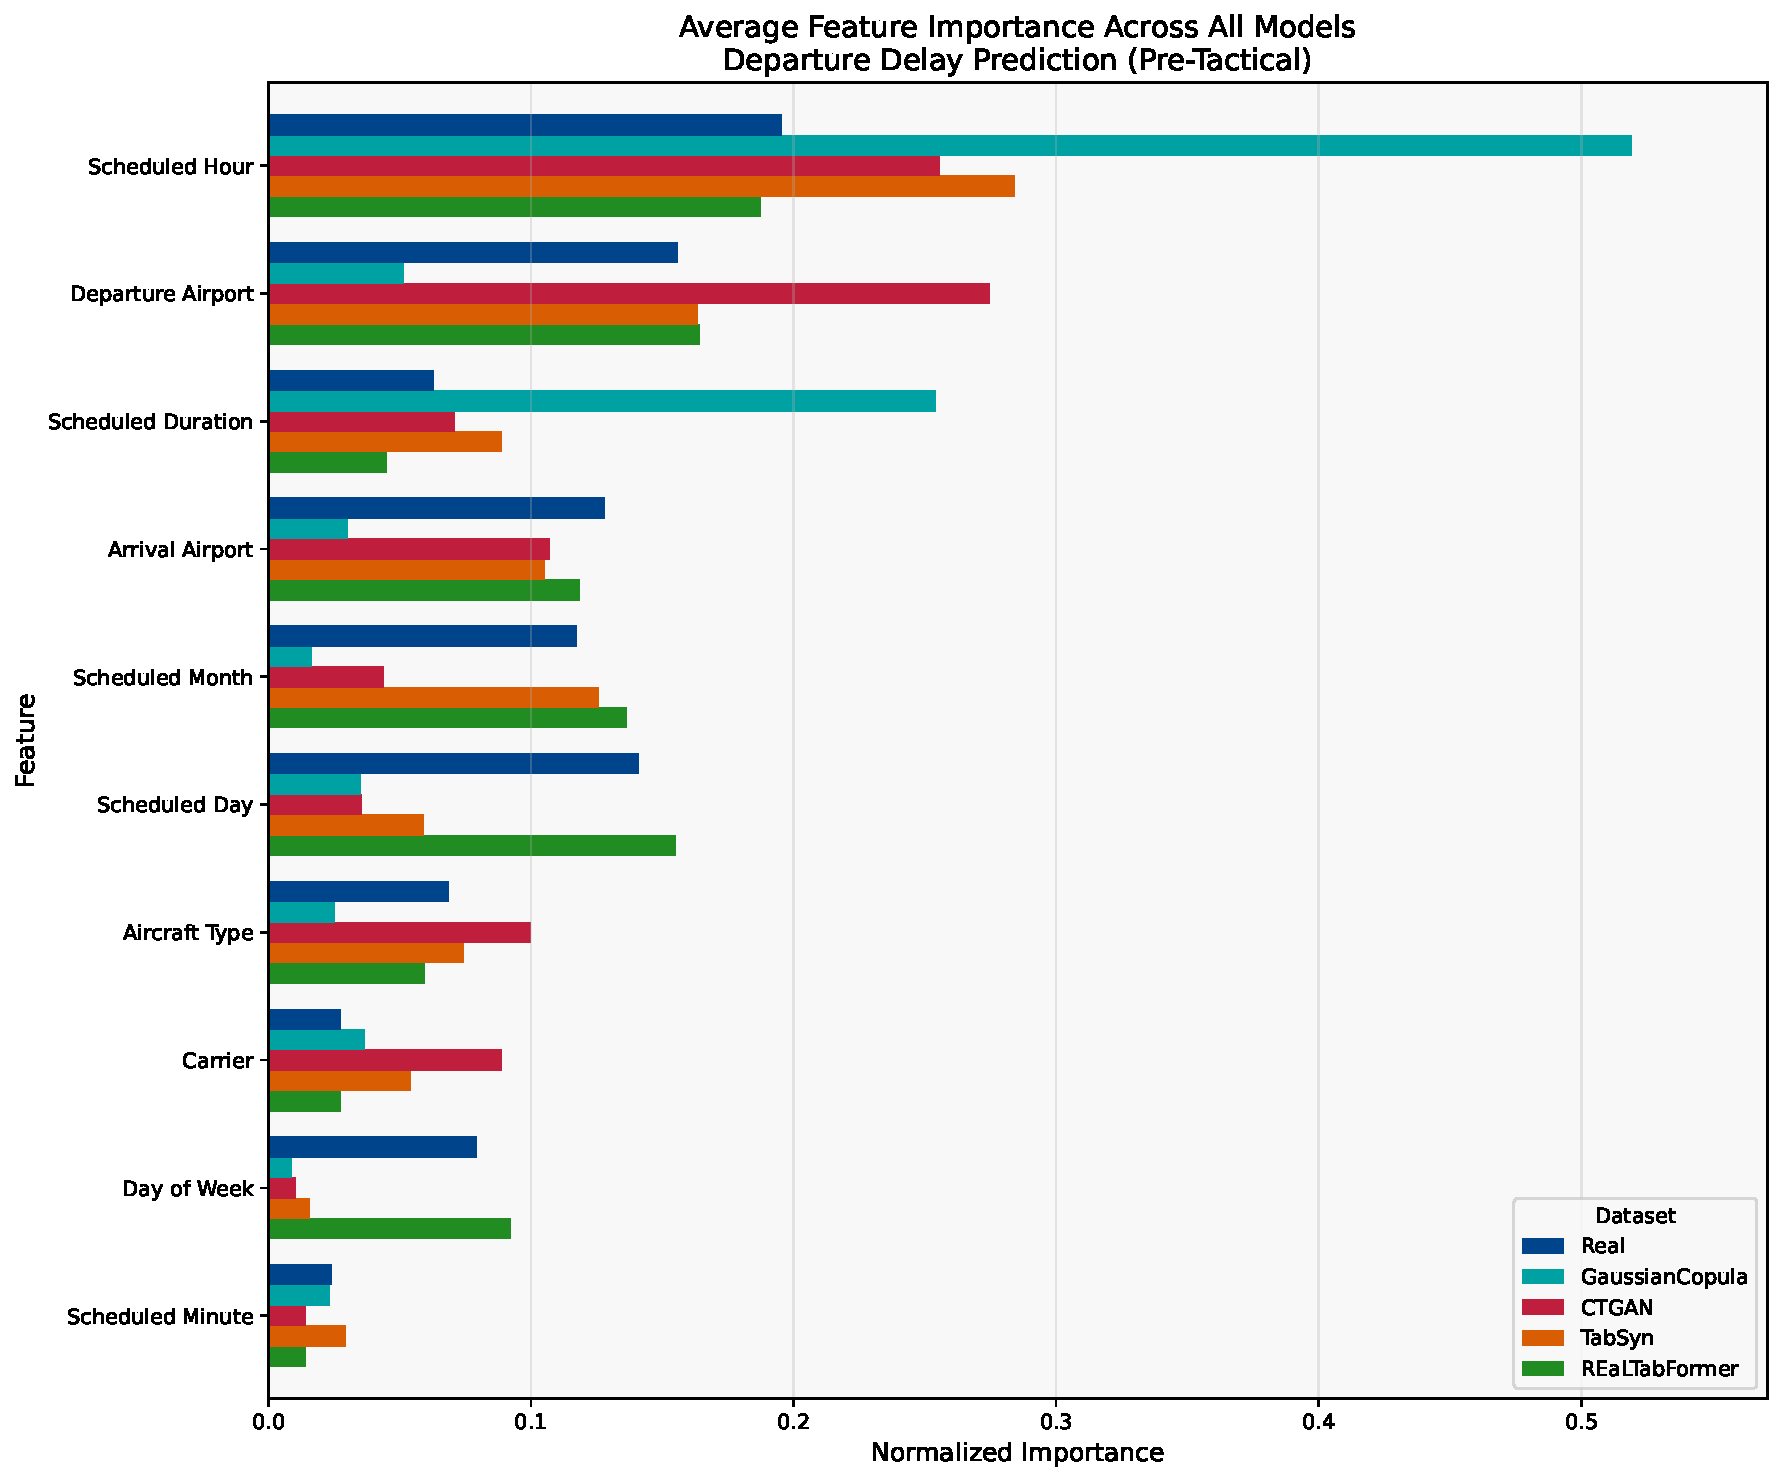
\includegraphics[width=\linewidth]{plots/departure_delay_min_pre-tactical/feature_importances/departure_delay_min_pre-tactical_all_models_feature_comparison.pdf}
    \caption{Feature importance comparison for pre-tactical departure delay prediction averaged across all models.}
    \label{fig:departure_features}
\end{figure}

The feature alignment analysis reveals interesting patterns (Figure~\ref{fig:departure_alignment}). While REaLTabFormer maintained near-perfect alignment (0.99), indicating that models trained on its synthetic data identify the same operational drivers as real-data models, Gaussian Copula's alignment dropped to 0.67. This misalignment could lead to incorrect operational conclusions if synthetic data users assume the same causal relationships present in real operations.

\begin{figure}[htbp]
    \centering
    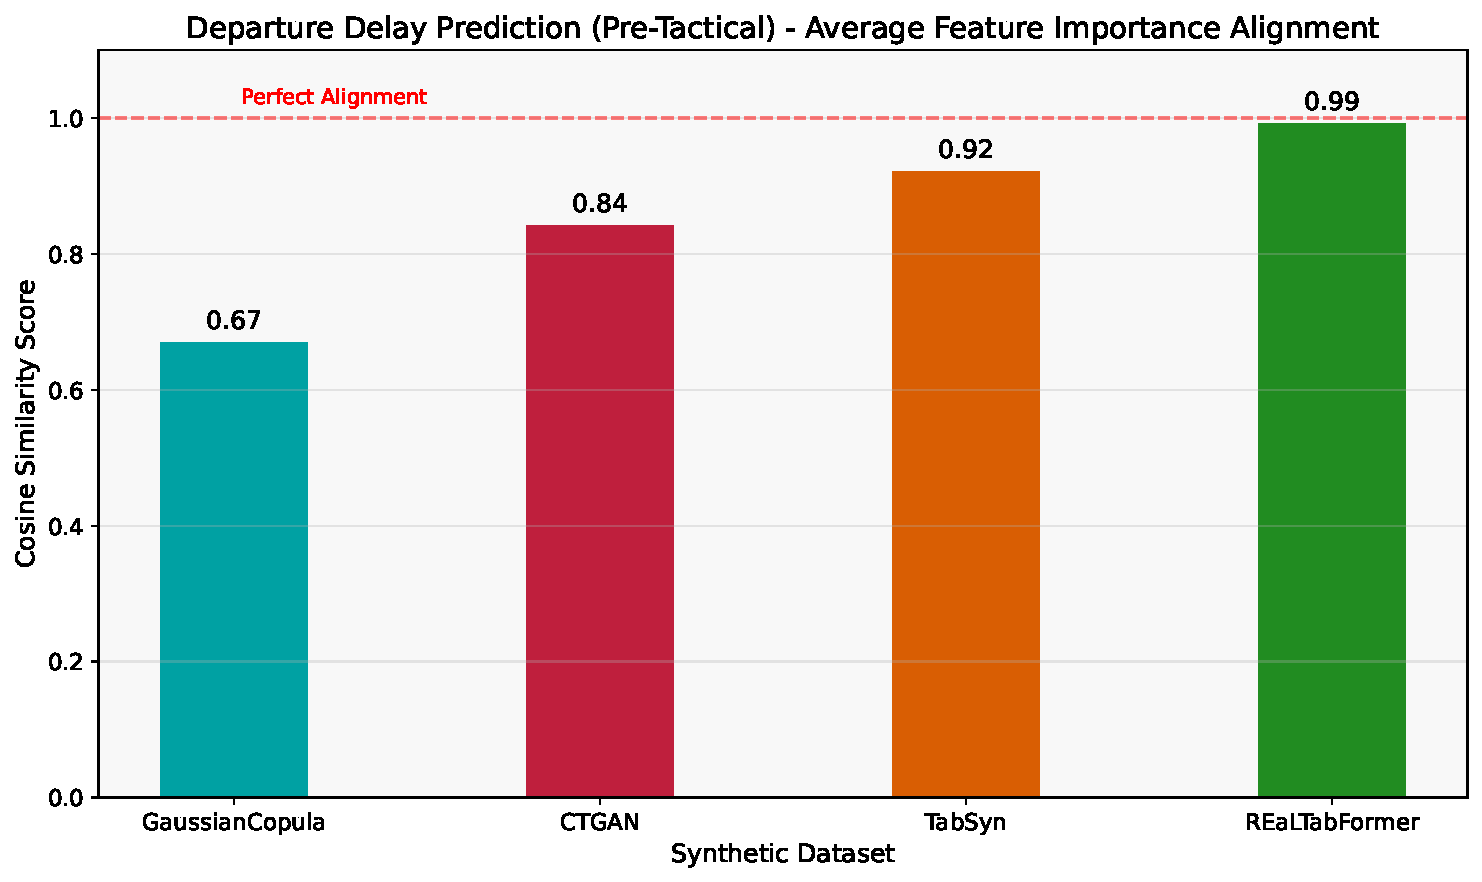
\includegraphics[width=0.8\linewidth]{plots/departure_delay_min_pre-tactical/departure_delay_min_pre-tactical_avg_alignment_score.pdf}
    \caption{Average feature importance alignment scores for pre-tactical departure delay prediction.}
    \label{fig:departure_alignment}
\end{figure}

\subsection{Arrival Delay Prediction}

Pre-tactical arrival delay prediction proved to be the most challenging task among all evaluated scenarios, with real-data R² values rarely exceeding 0.30 (Figure~\ref{fig:arrival_pre_r2}). This represents the cumulative uncertainty of multiple operational phases: ground operations affecting departure timing, en-route factors including air traffic congestion and weather, and destination airport conditions. The complexity of predicting arrival delays hours in advance using only scheduled information highlights fundamental limitations in aviation predictability.

\begin{figure}[htbp]
    \centering
    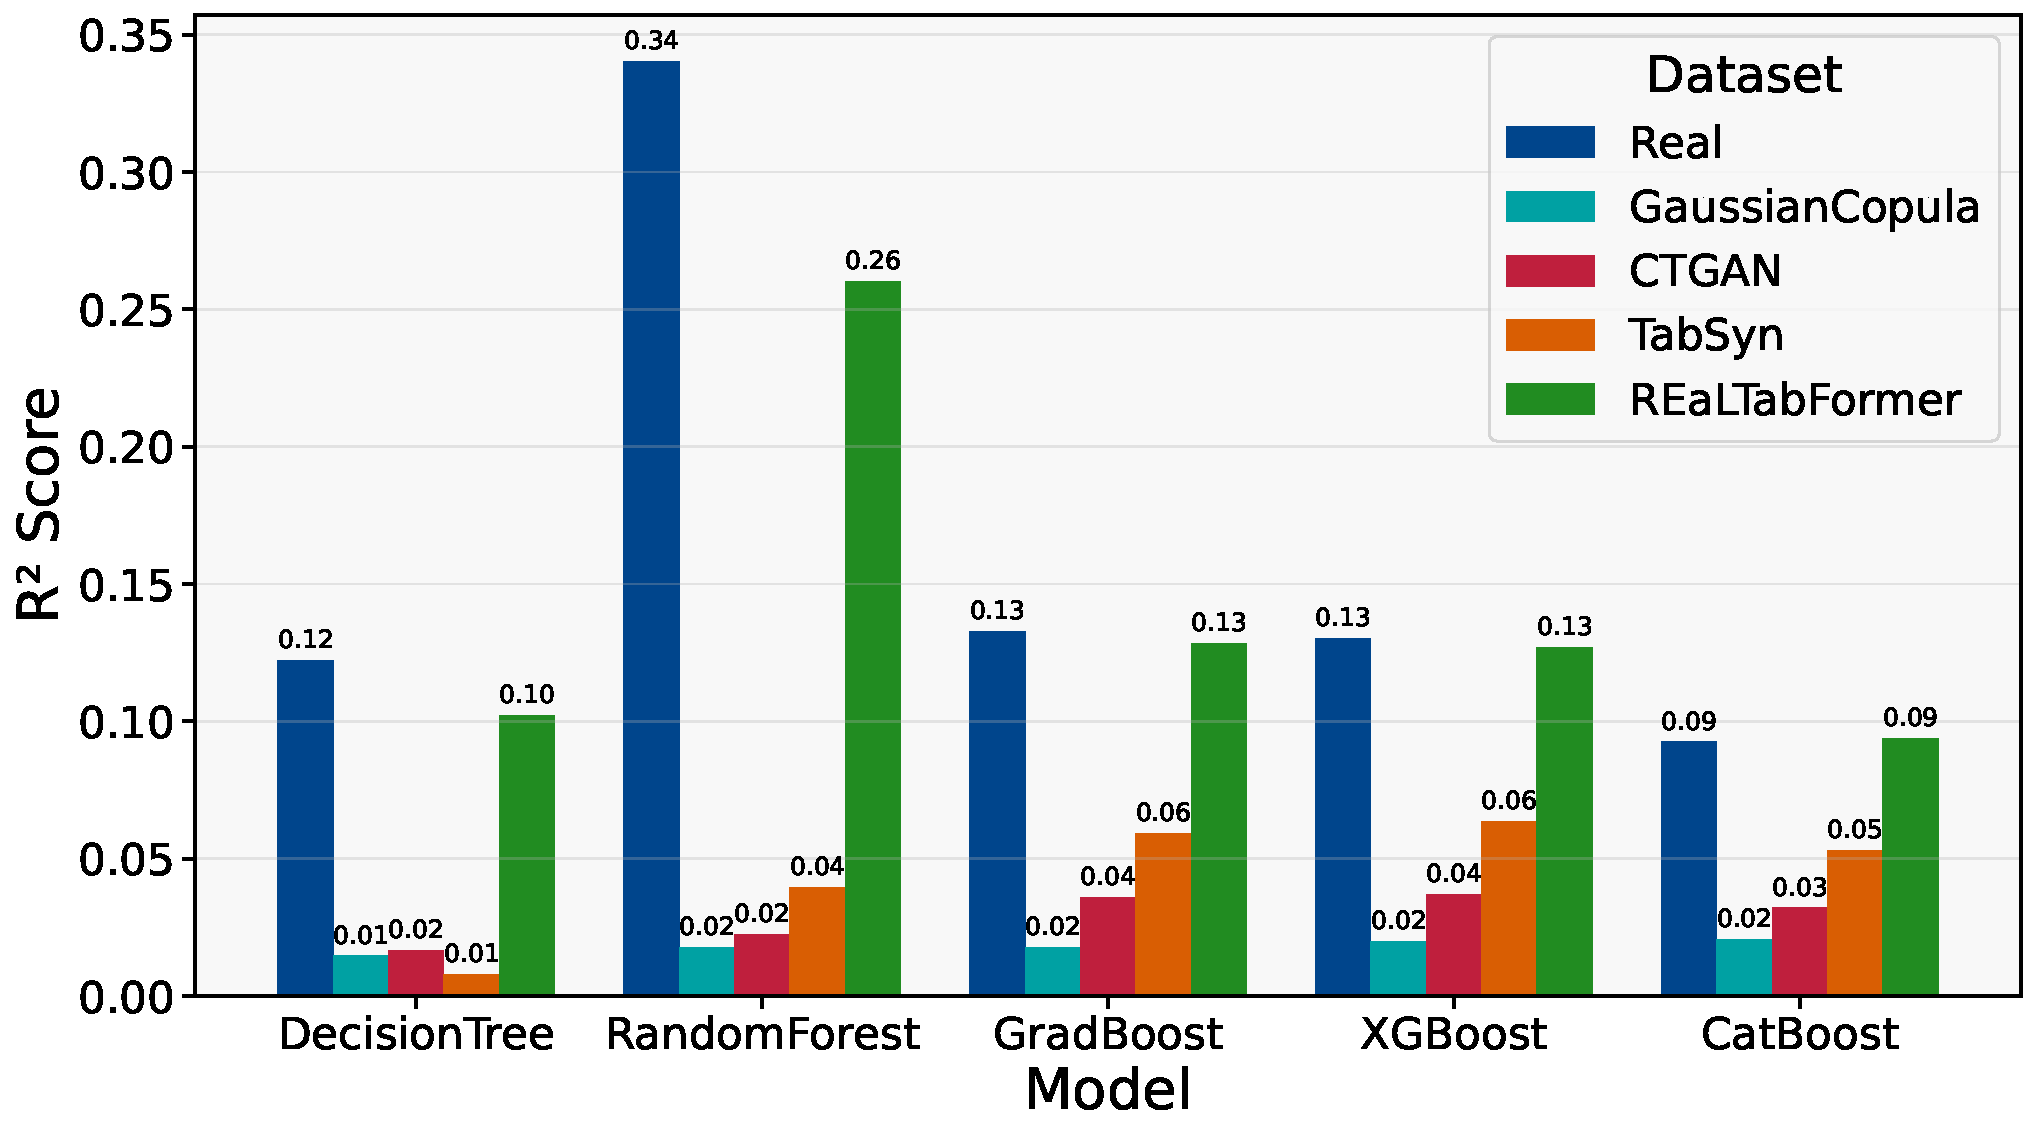
\includegraphics[width=\linewidth]{plots/arrival_delay_min_pre-tactical/arrival_delay_min_pre-tactical_r2.pdf}
    \caption{Coefficient of determination (R²) for pre-tactical arrival delay prediction across different models and synthetic data generators.}
    \label{fig:arrival_pre_r2}
\end{figure}

The error metrics demonstrate that even under these challenging conditions, synthetic data generators maintained their relative performance hierarchy (Figures~\ref{fig:arrival_pre_rmse} and \ref{fig:arrival_pre_mae}). REaLTabFormer continued to achieve the lowest error rates. Thus, the transformer architecture's advantage becomes more pronounced in complex scenarios where capturing subtle interactions between multiple categorical and temporal features proves crucial.

\begin{figure}[htbp]
    \centering
    \begin{subfigure}[b]{0.49\textwidth}
        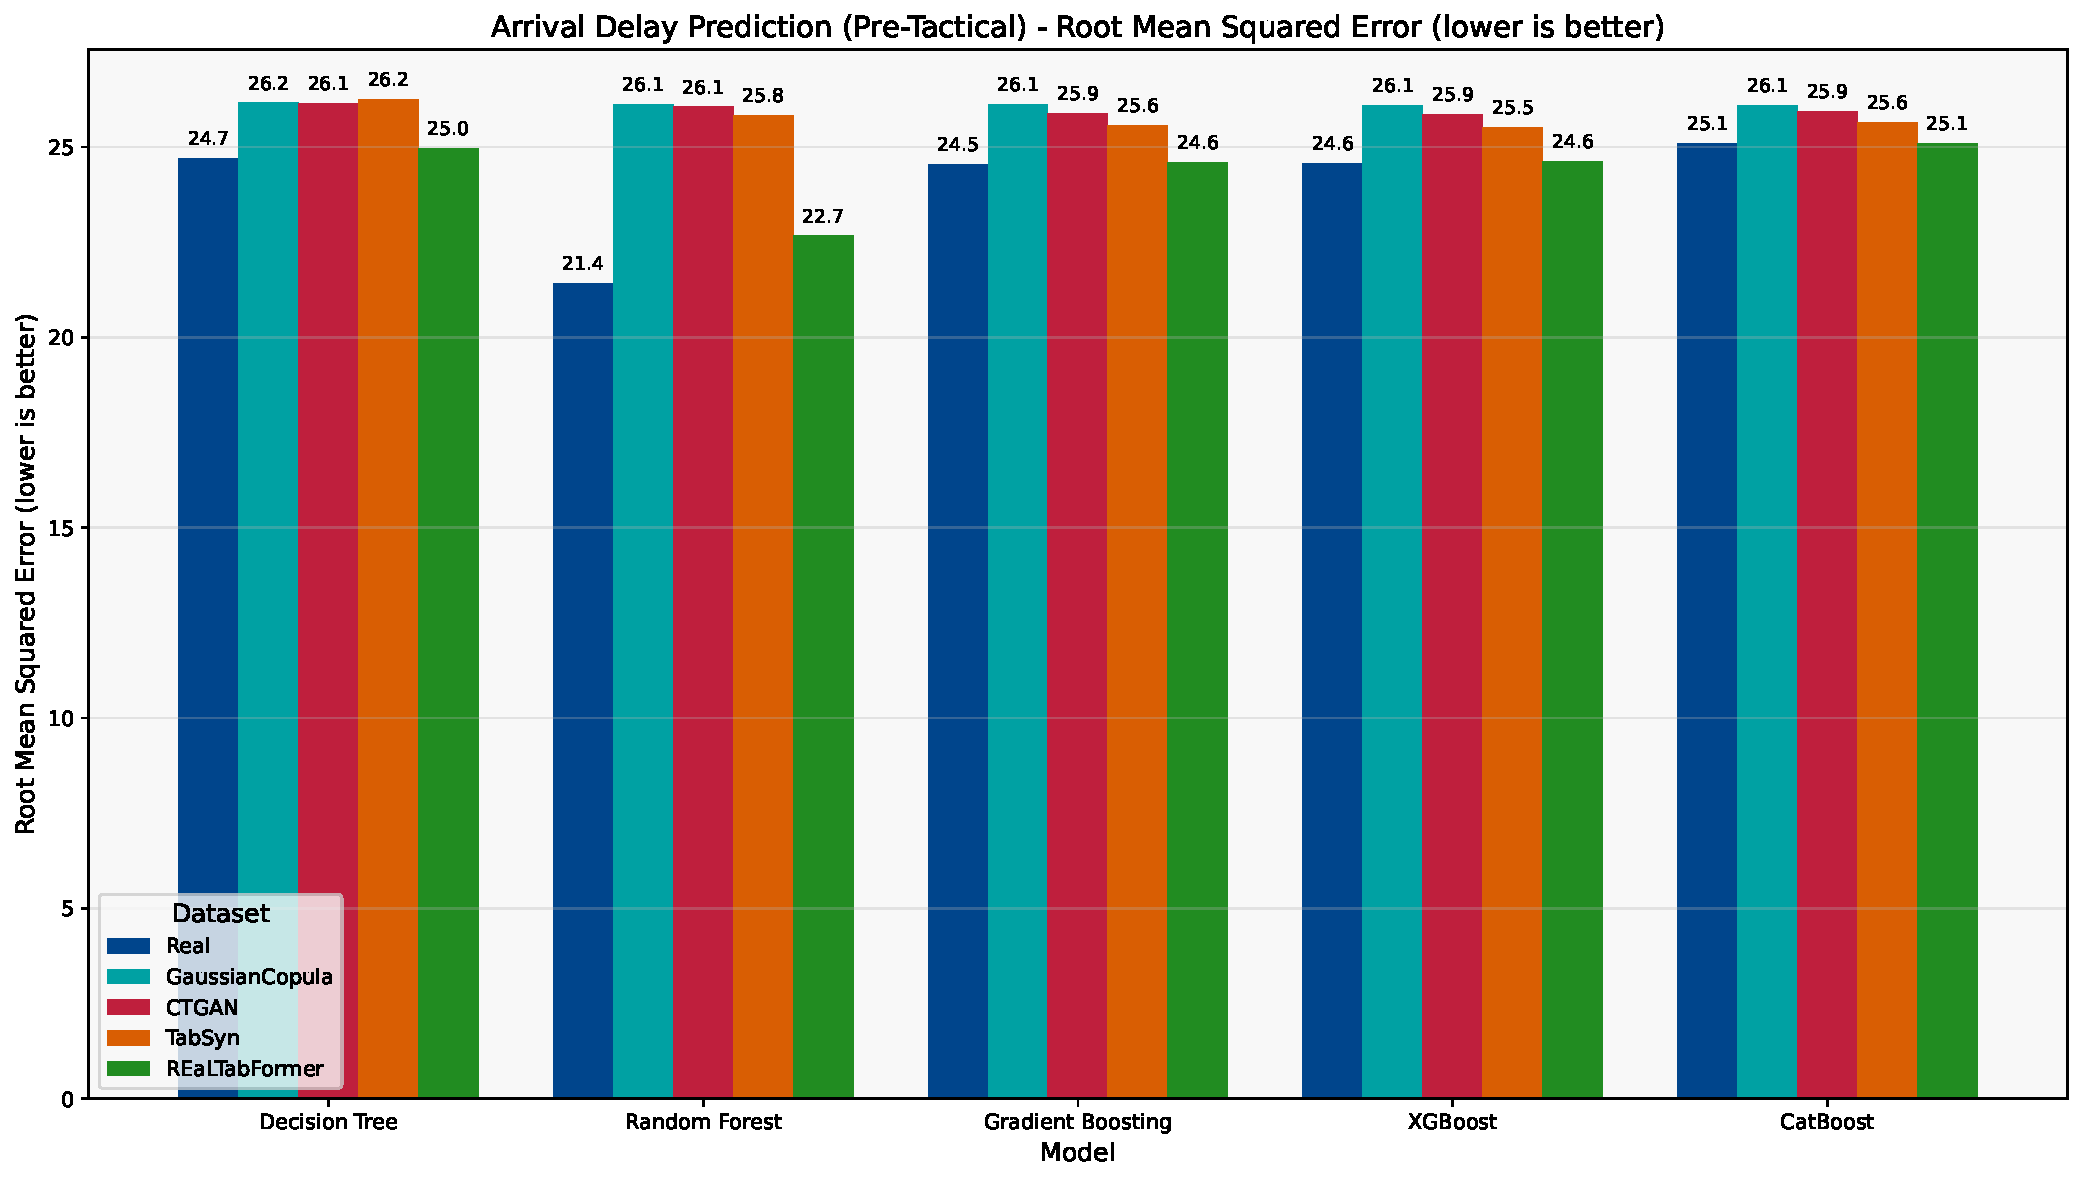
\includegraphics[width=\linewidth]{plots/arrival_delay_min_pre-tactical/arrival_delay_min_pre-tactical_rmse.pdf}
        \caption{Root Mean Squared Error}
        \label{fig:arrival_pre_rmse}
    \end{subfigure}
    \hfill
    \begin{subfigure}[b]{0.49\textwidth}
        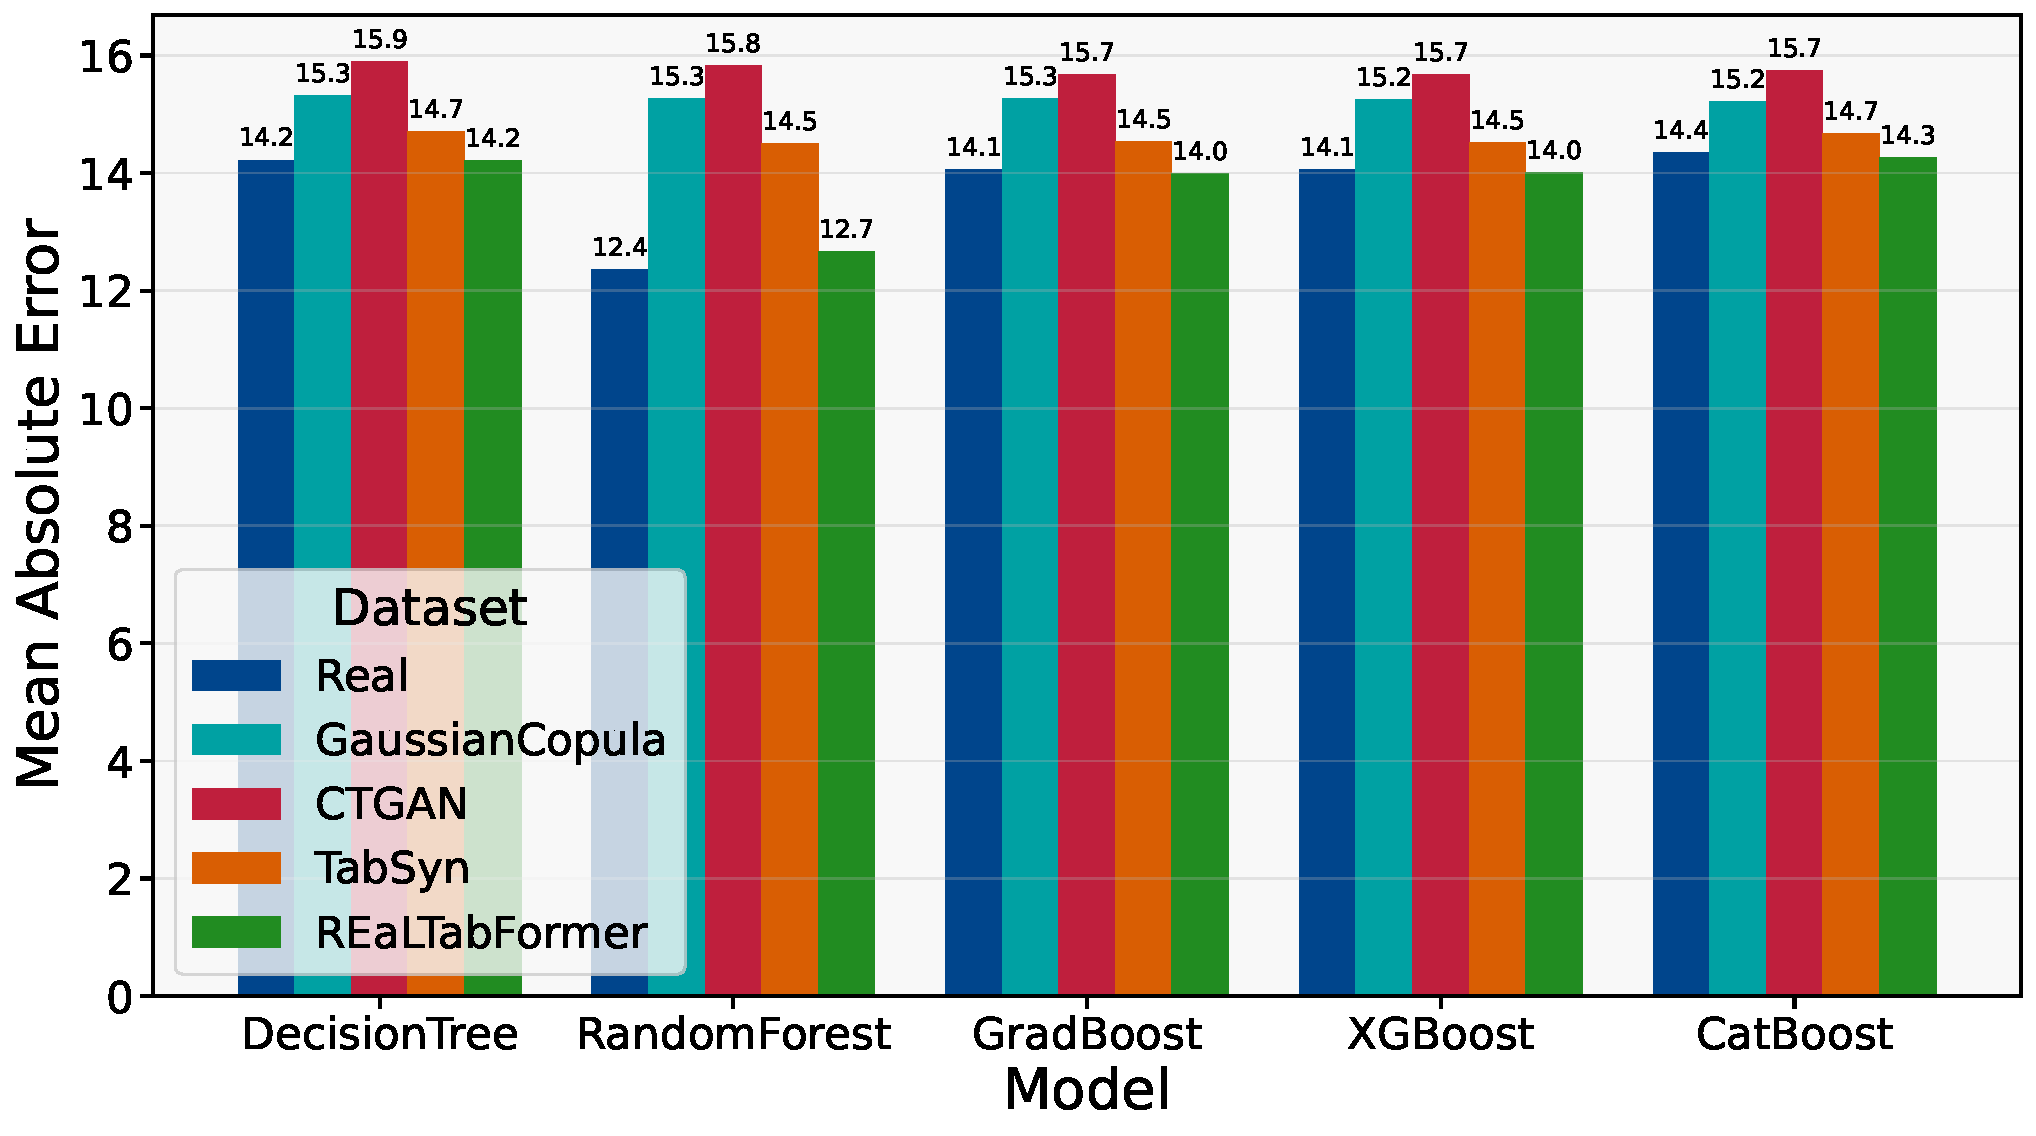
\includegraphics[width=\linewidth]{plots/arrival_delay_min_pre-tactical/arrival_delay_min_pre-tactical_mae.pdf}
        \caption{Mean Absolute Error}
        \label{fig:arrival_pre_mae}
    \end{subfigure}
    \caption{Prediction error metrics for pre-tactical arrival delay across models and synthetic data generators.}
\end{figure}

Despite the increased task complexity, REaLTabFormer maintained  utility performance at 0.95 (Figure~\ref{fig:arrival_pre_utility}), demonstrating robustness across different prediction scenarios. This consistency suggests that the transformer-based approach successfully captures the underlying statistical structure that relates scheduled flight information to eventual arrival performance, even when that relationship becomes increasingly attenuated by intervening factors.

\begin{figure}[htbp]
    \centering
    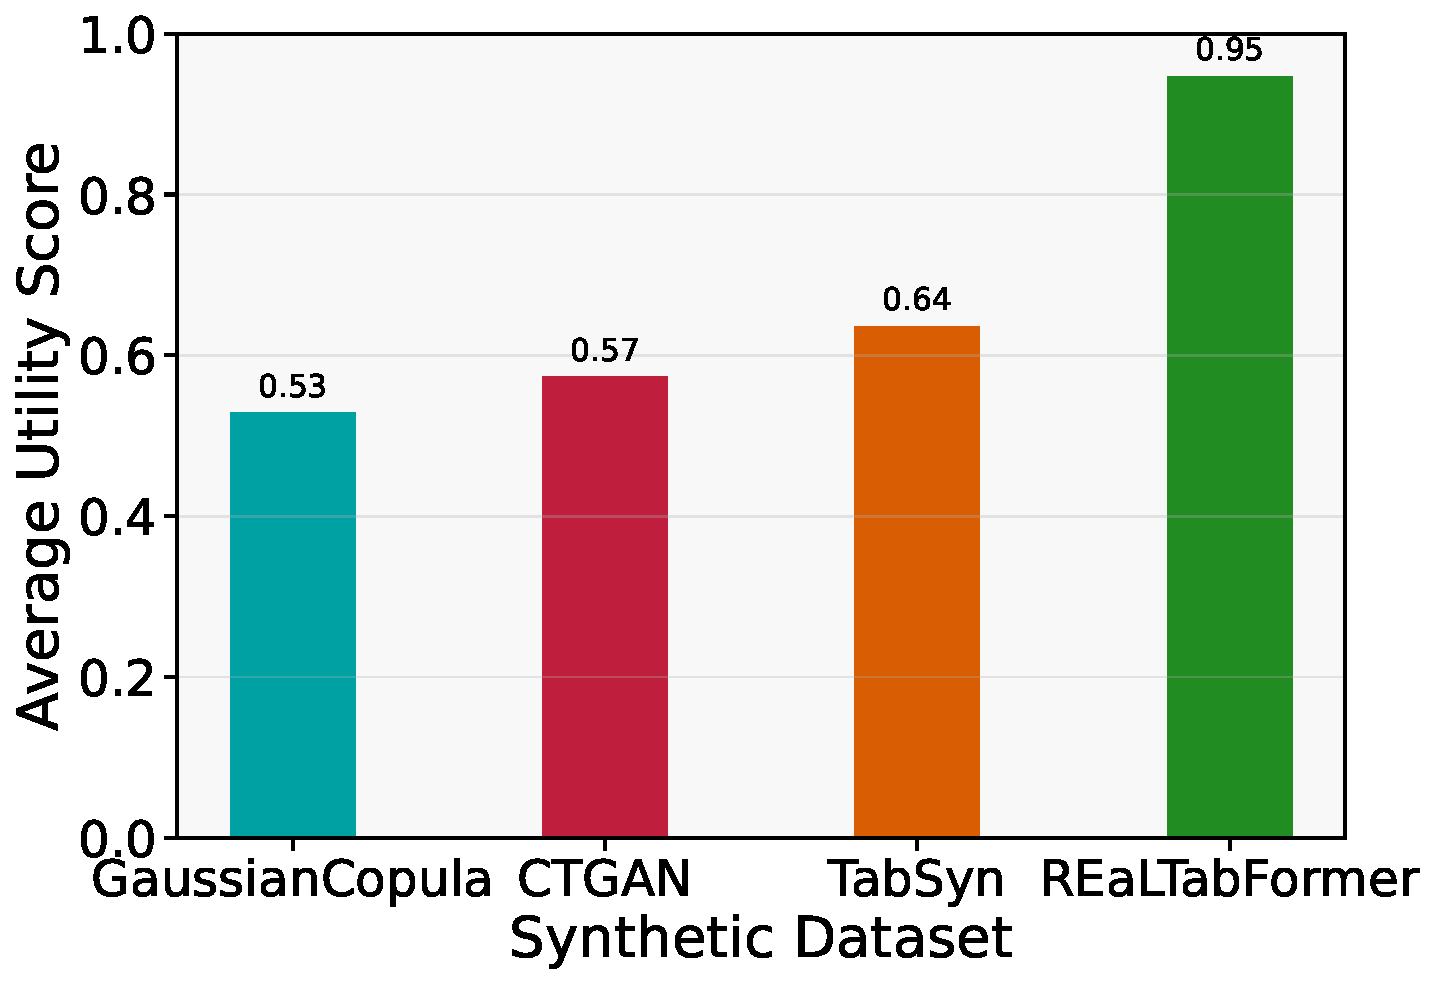
\includegraphics[width=0.8\linewidth]{plots/arrival_delay_min_pre-tactical/arrival_delay_min_pre-tactical_avg_utility.pdf}
    \caption{Average utility scores for pre-tactical arrival delay prediction across synthetic data generators.}
    \label{fig:arrival_pre_utility}
\end{figure}

Feature importance analysis for arrival delays revealed more complex patterns than departure delay prediction (Figure~\ref{fig:arrival_features}). Scheduled flight duration emerged as an additional significant predictor alongside temporal and airport features, reflecting the reality that longer flights have more opportunities for en-route delays and recovery. The distribution of importance across multiple features indicates that arrival delay prediction requires modeling interactions between temporal, spatial, and operational characteristics simultaneously.

\begin{figure}[htbp]
    \centering
    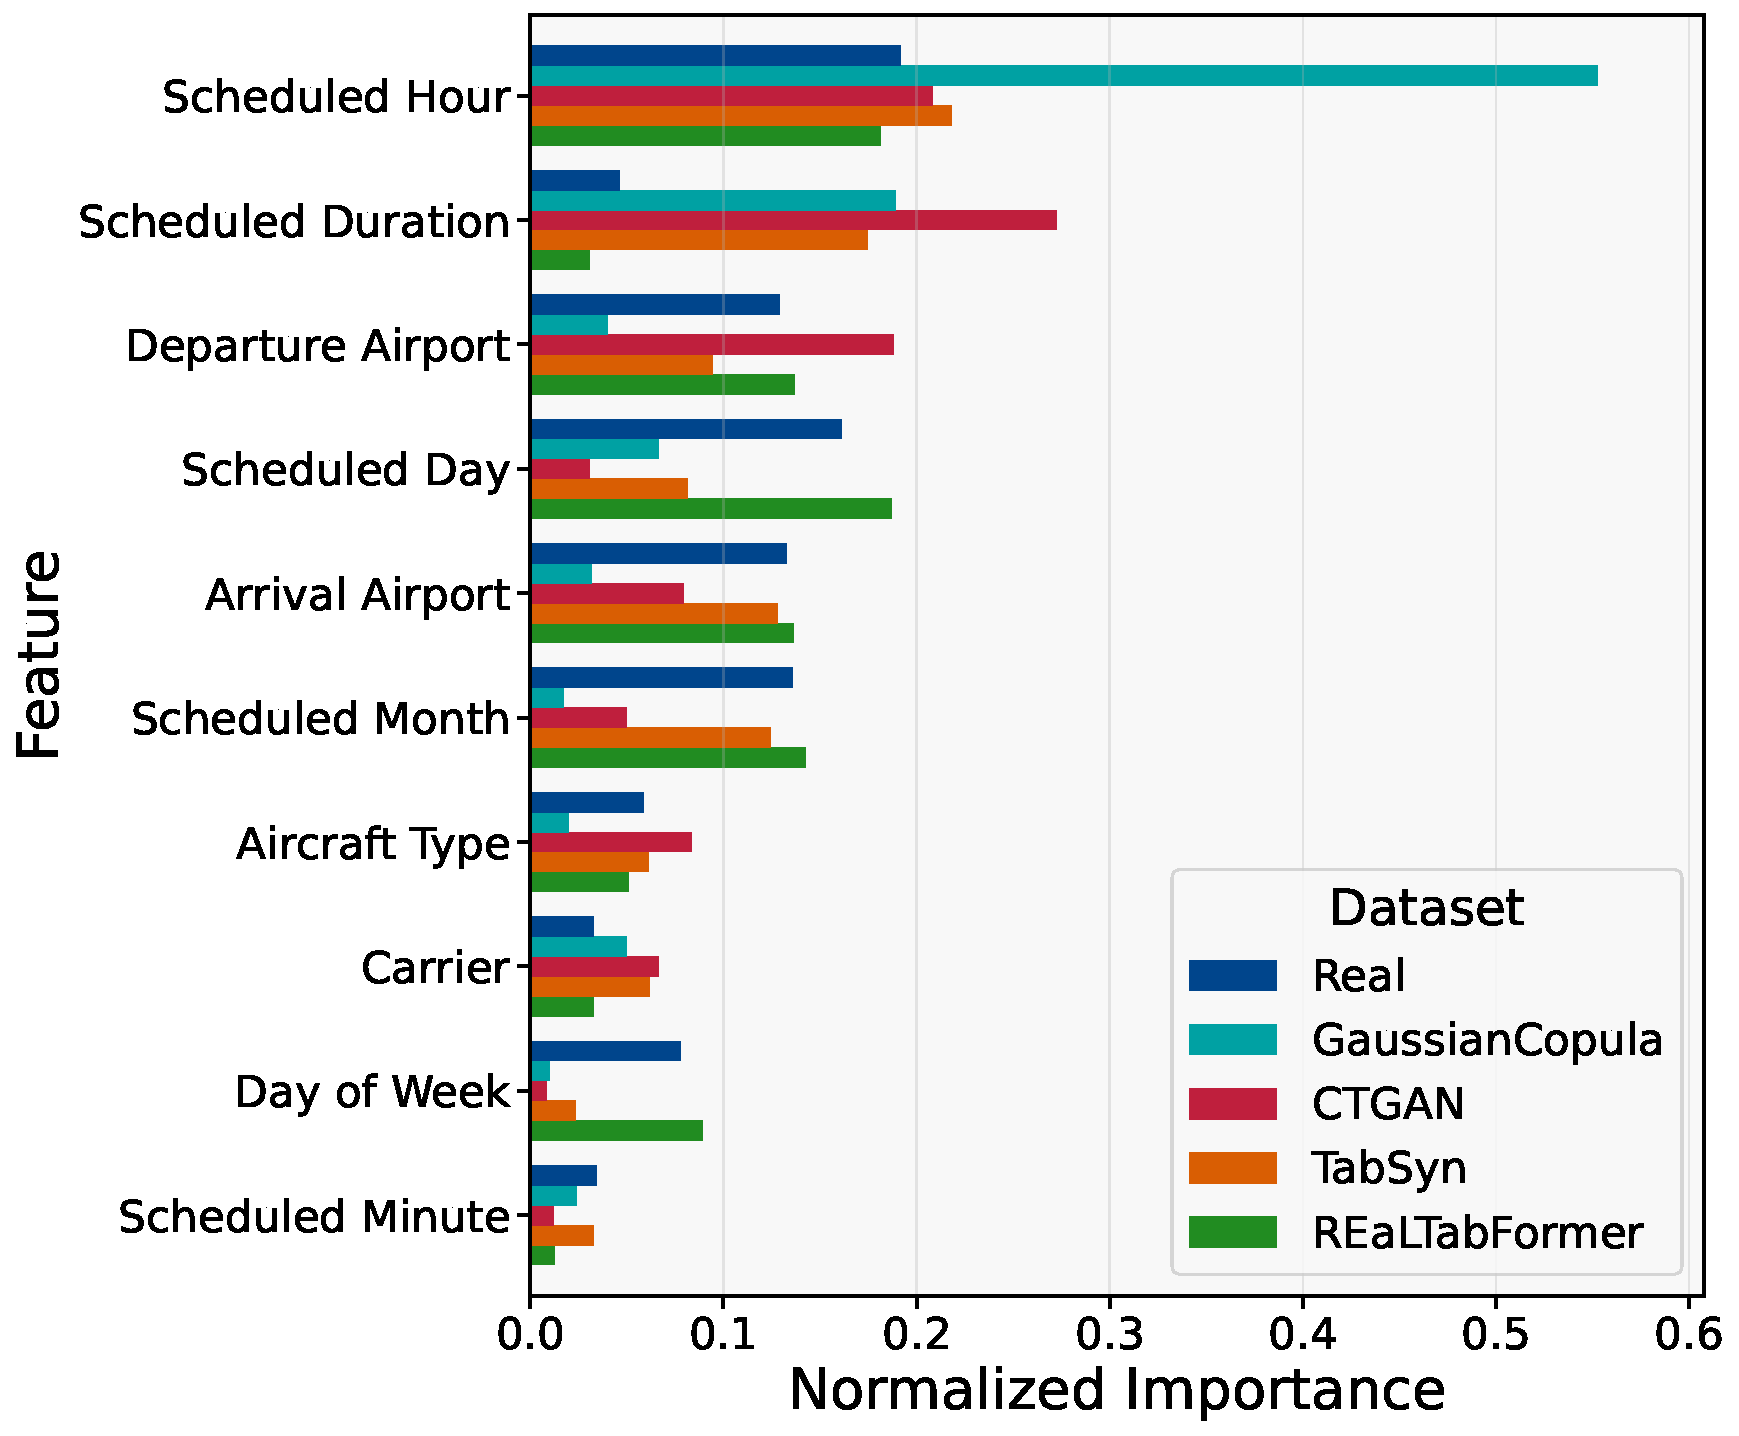
\includegraphics[width=\linewidth]{plots/arrival_delay_min_pre-tactical/feature_importances/arrival_delay_min_pre-tactical_all_models_feature_comparison.pdf}
    \caption{Feature importance comparison for pre-tactical arrival delay prediction averaged across all models.}
    \label{fig:arrival_features}
\end{figure}

The feature alignment scores maintained the established pattern, with REaLTabFormer achieving near-perfect alignment (0.99) while simpler methods showed progressive degradation (Figure~\ref{fig:arrival_alignment}). This consistency in feature relationship preservation across increasingly difficult tasks demonstrates REaLTabFormer's fundamental advantage in capturing the complex dependencies present in aviation operational data.

\begin{figure}[htbp]
    \centering
    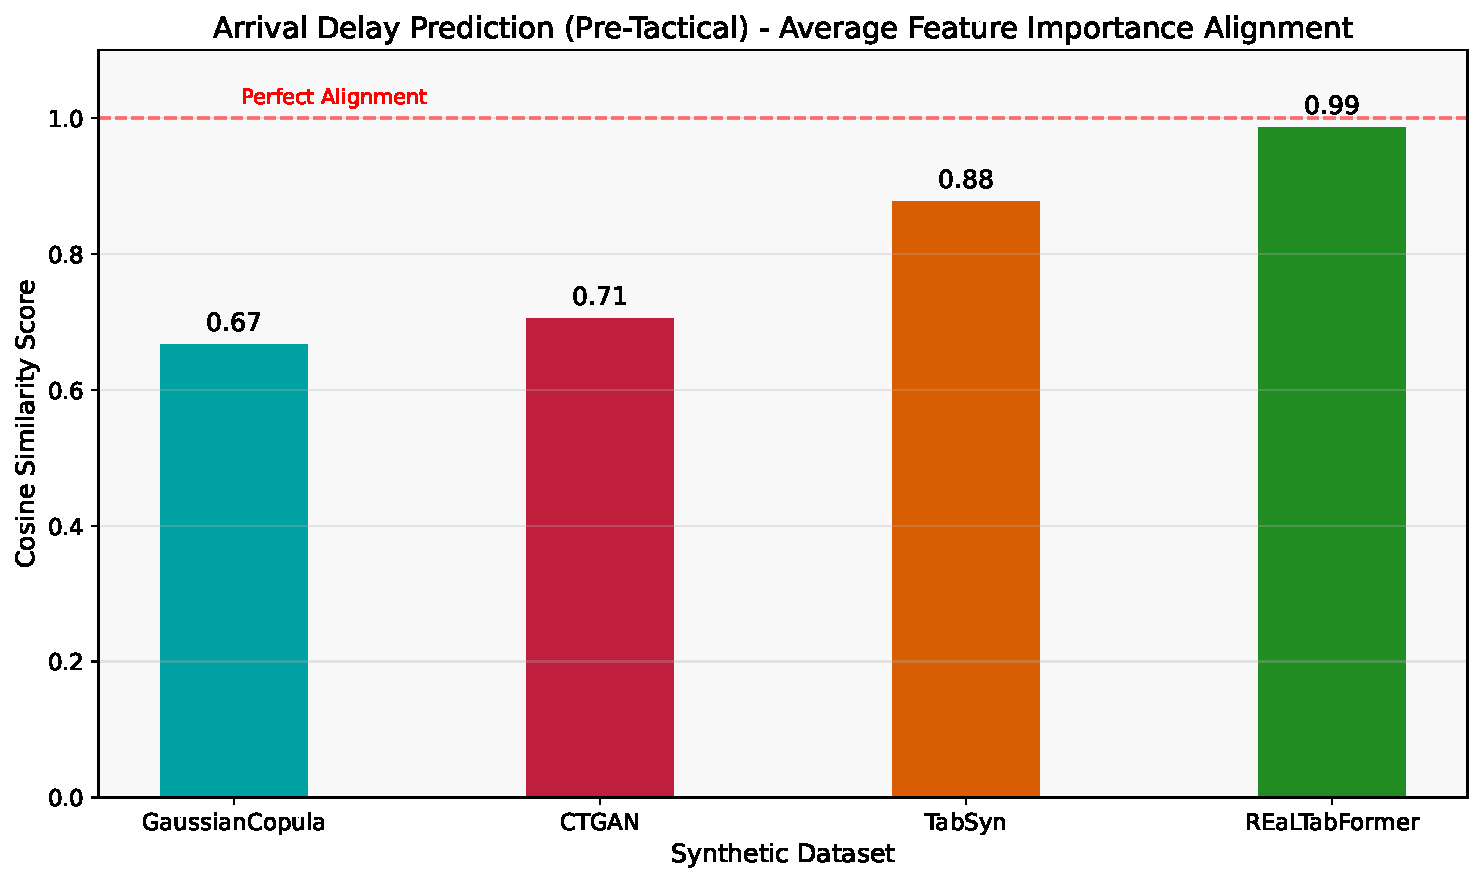
\includegraphics[width=0.8\linewidth]{plots/arrival_delay_min_pre-tactical/arrival_delay_min_pre-tactical_avg_alignment_score.pdf}
    \caption{Average feature importance alignment scores for pre-tactical arrival delay prediction.}
    \label{fig:arrival_alignment}
\end{figure}

\subsection{Turnaround Time Prediction}

Turnaround time prediction in pre-tactical mode demonstrated the highest predictability among all evaluated tasks, with real-data models achieving R² values between 0.27-0.44 (Figure~\ref{fig:turnaround_pre_r2}). This performance likely reflects the more deterministic nature of turnaround processes compared to delay propagation. While external factors certainly influence turnaround times, the core processes—passenger deplaning, cleaning, catering, fueling, and boarding—follow more predictable patterns based on aircraft type, airport facilities, and scheduled timing.

\begin{figure}[htbp]
    \centering
    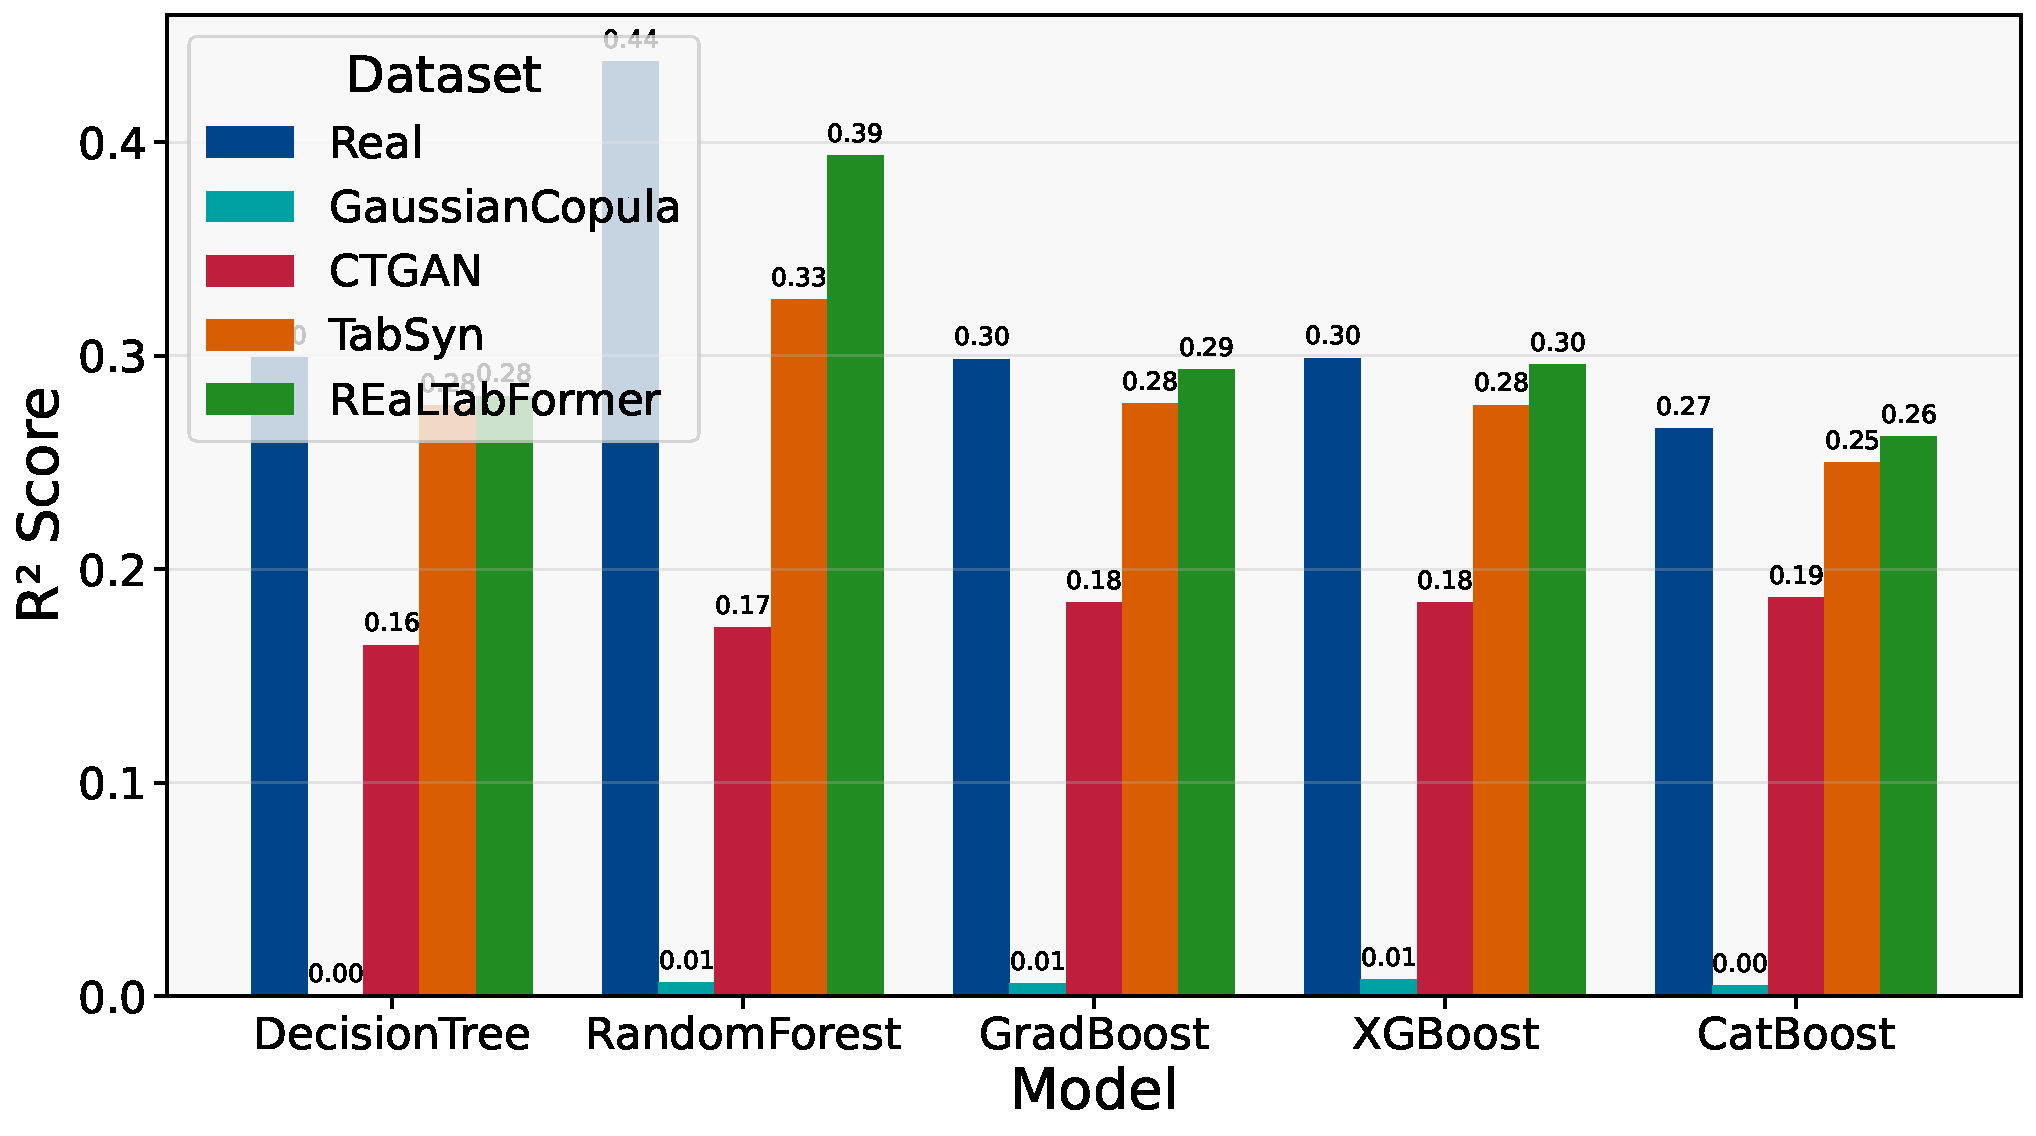
\includegraphics[width=\linewidth]{plots/turnaround_min_pre-tactical/turnaround_min_pre-tactical_r2.pdf}
    \caption{Coefficient of determination (R²) for pre-tactical turnaround time prediction across different models and synthetic data generators.}
    \label{fig:turnaround_pre_r2}
\end{figure}

The error metrics revealed pronounced performance differences between synthetic generators (Figures~\ref{fig:turnaround_pre_rmse} and \ref{fig:turnaround_pre_mae}). REaLTabFormer achieved RMSE values within 3\% of real-data baselines, demonstrating preservation of the predictive relationships between scheduled characteristics and turnaround requirements. TabSyn followed closely, while CTGAN showed moderate degradation and Gaussian Copula exhibited substantial performance gaps.

\begin{figure}[htbp]
    \centering
    \begin{subfigure}[b]{0.49\textwidth}
        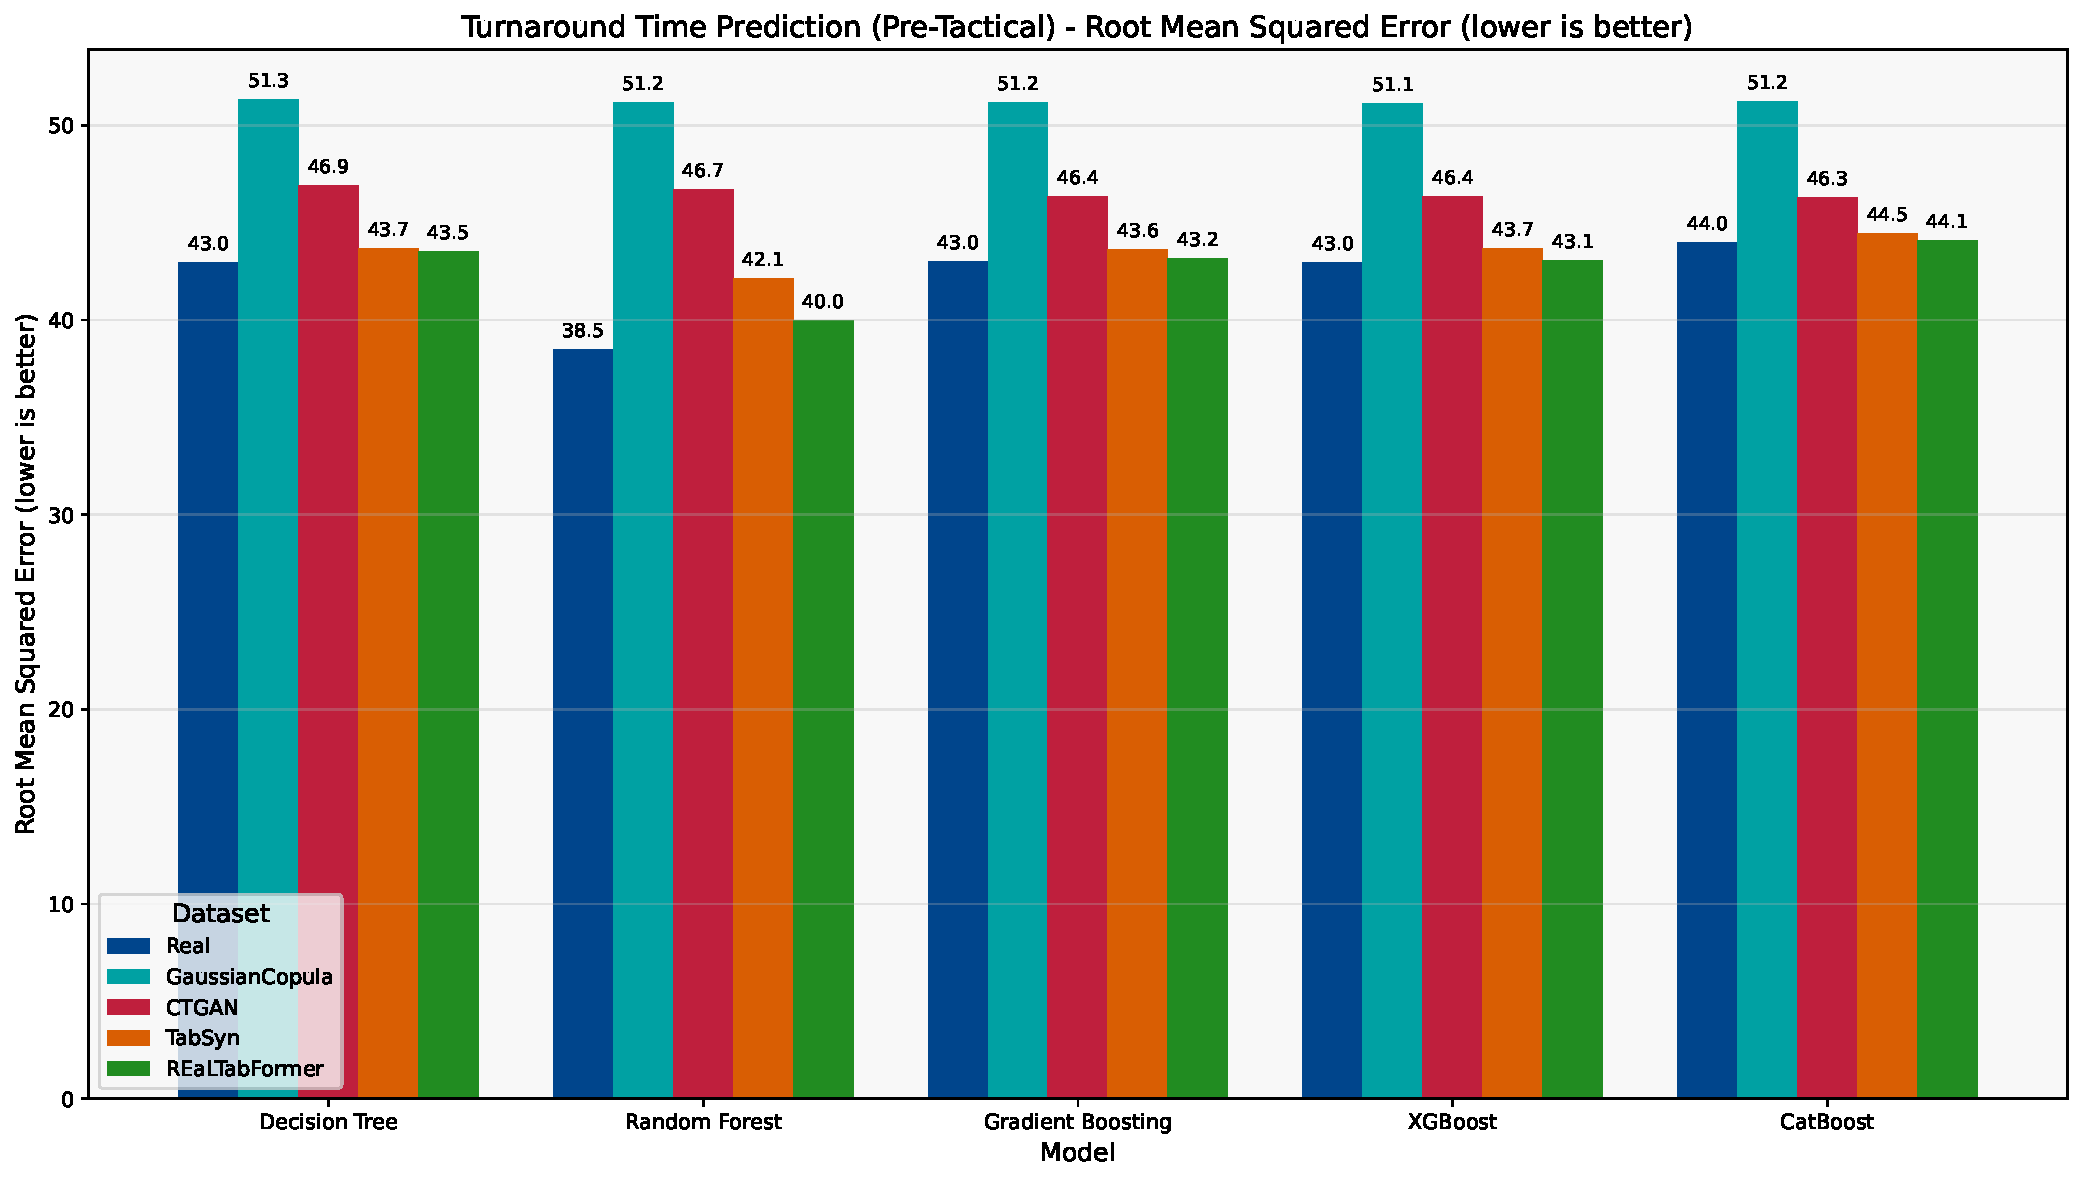
\includegraphics[width=\linewidth]{plots/turnaround_min_pre-tactical/turnaround_min_pre-tactical_rmse.pdf}
        \caption{Root Mean Squared Error}
        \label{fig:turnaround_pre_rmse}
    \end{subfigure}
    \hfill
    \begin{subfigure}[b]{0.49\textwidth}
        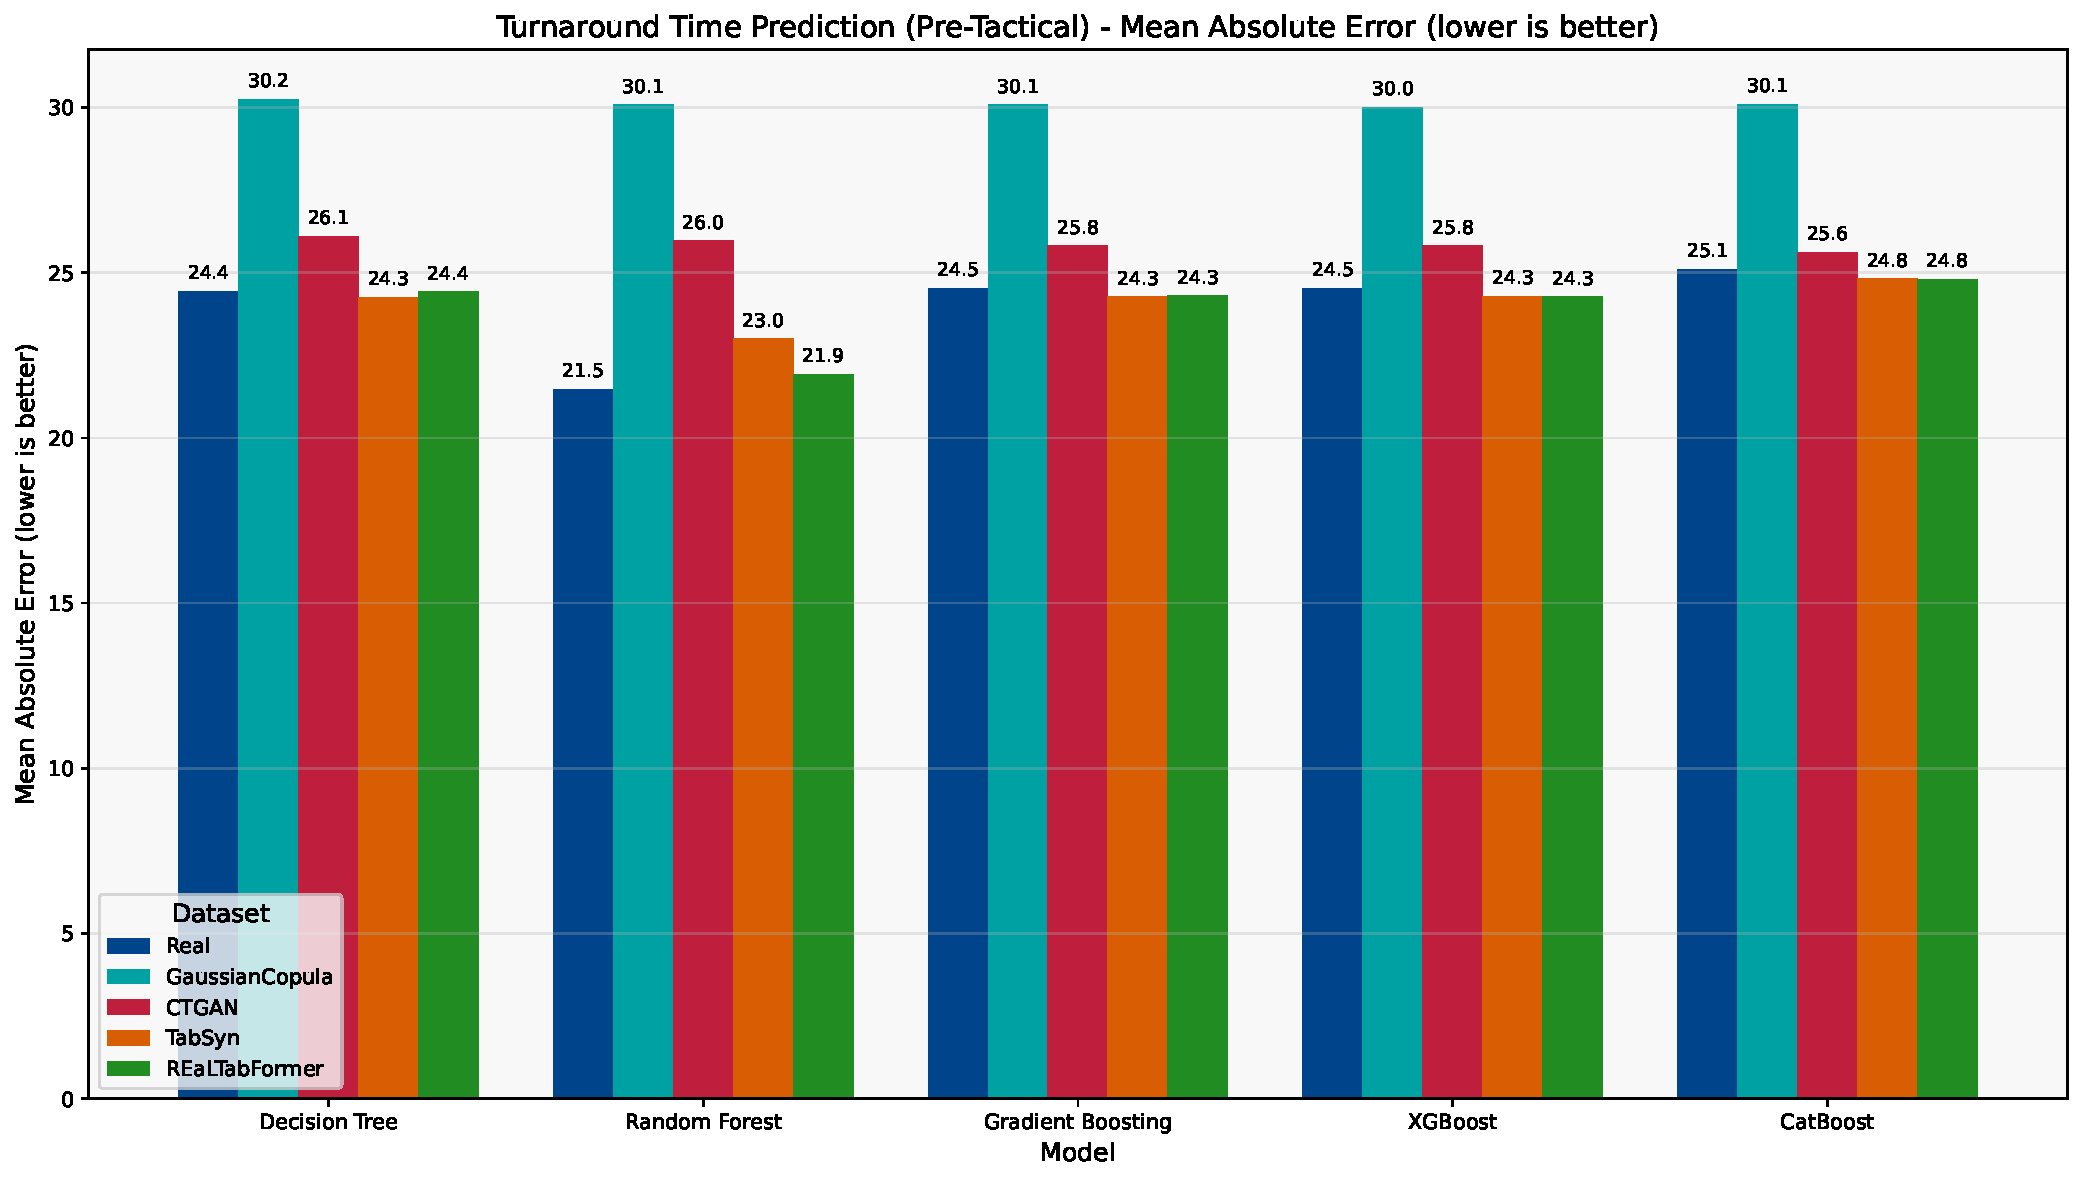
\includegraphics[width=\linewidth]{plots/turnaround_min_pre-tactical/turnaround_min_pre-tactical_mae.pdf}
        \caption{Mean Absolute Error}
        \label{fig:turnaround_pre_mae}
    \end{subfigure}
    \caption{Prediction error metrics for pre-tactical turnaround time across models and synthetic data generators.}
\end{figure}

The utility score analysis confirmed turnaround prediction as the most successful application of synthetic data (Figure~\ref{fig:turnaround_pre_utility}). REaLTabFormer achieved a utility score of 0.97, followed by TabSyn at 0.93. These high scores indicate that for the critical operational task of turnaround planning, synthetic data can serve as an effective substitute for proprietary operational records, enabling advanced analytics capabilities for organizations without access to comprehensive historical datasets.

\begin{figure}[htbp]
    \centering
    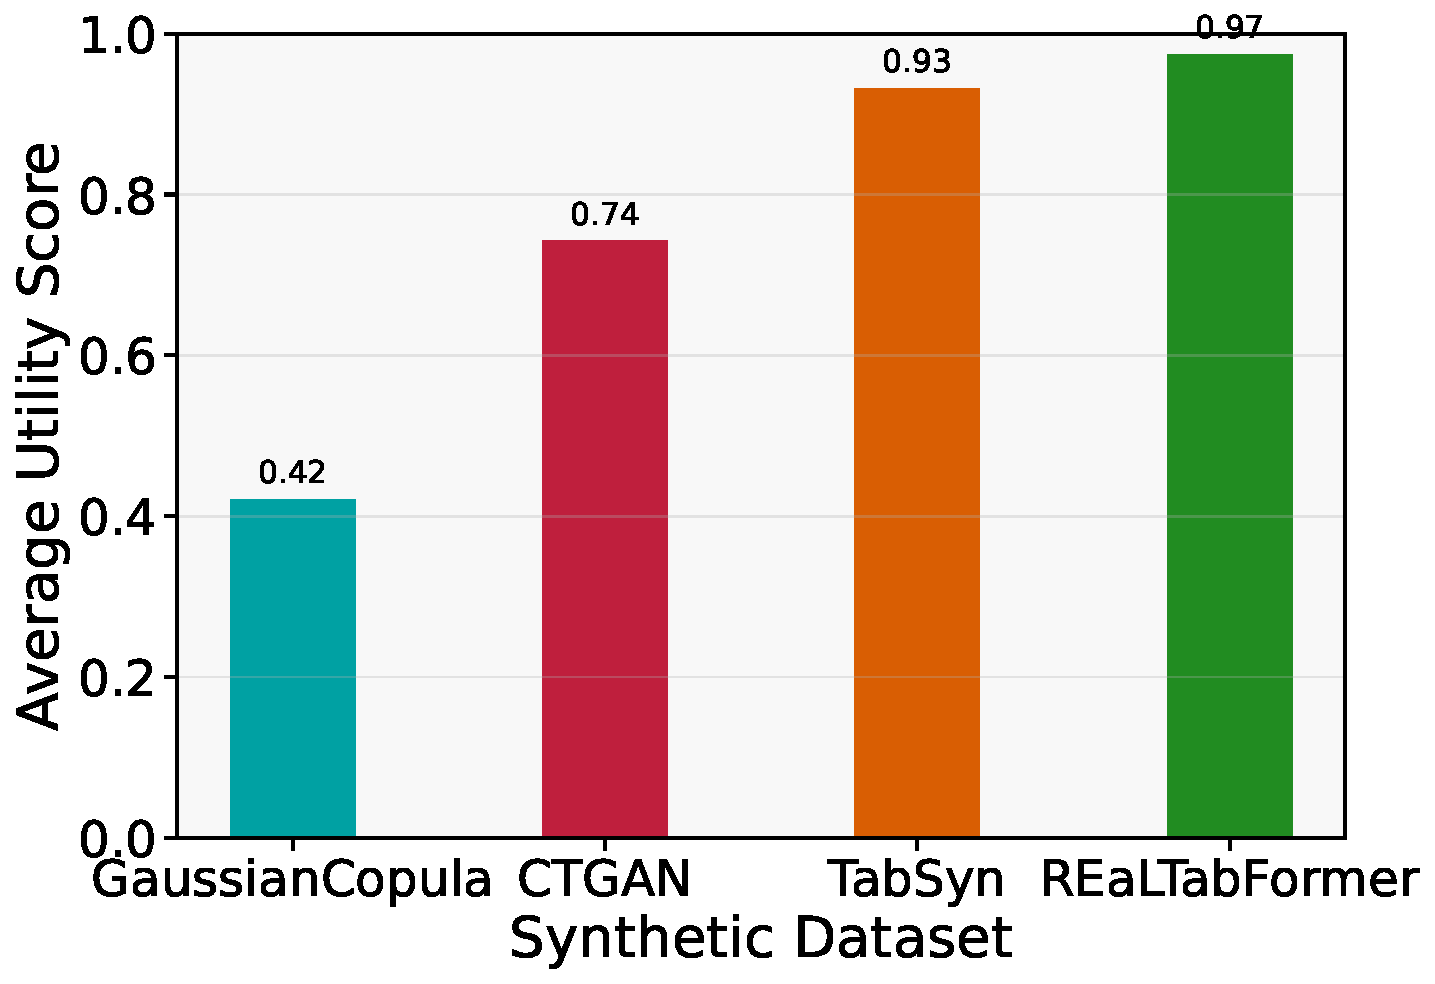
\includegraphics[width=0.8\linewidth]{plots/turnaround_min_pre-tactical/turnaround_min_pre-tactical_avg_utility.pdf}
    \caption{Average utility scores for pre-tactical turnaround time prediction across synthetic data generators.}
    \label{fig:turnaround_pre_utility}
\end{figure}

Feature importance analysis revealed that scheduled hour/Duration and airport identifiers emerged as the dominant predictors across all data sources (Figure~\ref{fig:turnaround_pre_features}). This pattern aligns with operational knowledge: turnaround processes exhibit significant time-of-day variations due to staffing levels, gate availability, and passenger flow patterns. Airport-specific effects capture differences in terminal layouts, ground handling procedures, and infrastructure constraints that systematically influence turnaround efficiency.

\begin{figure}[htbp]
    \centering
    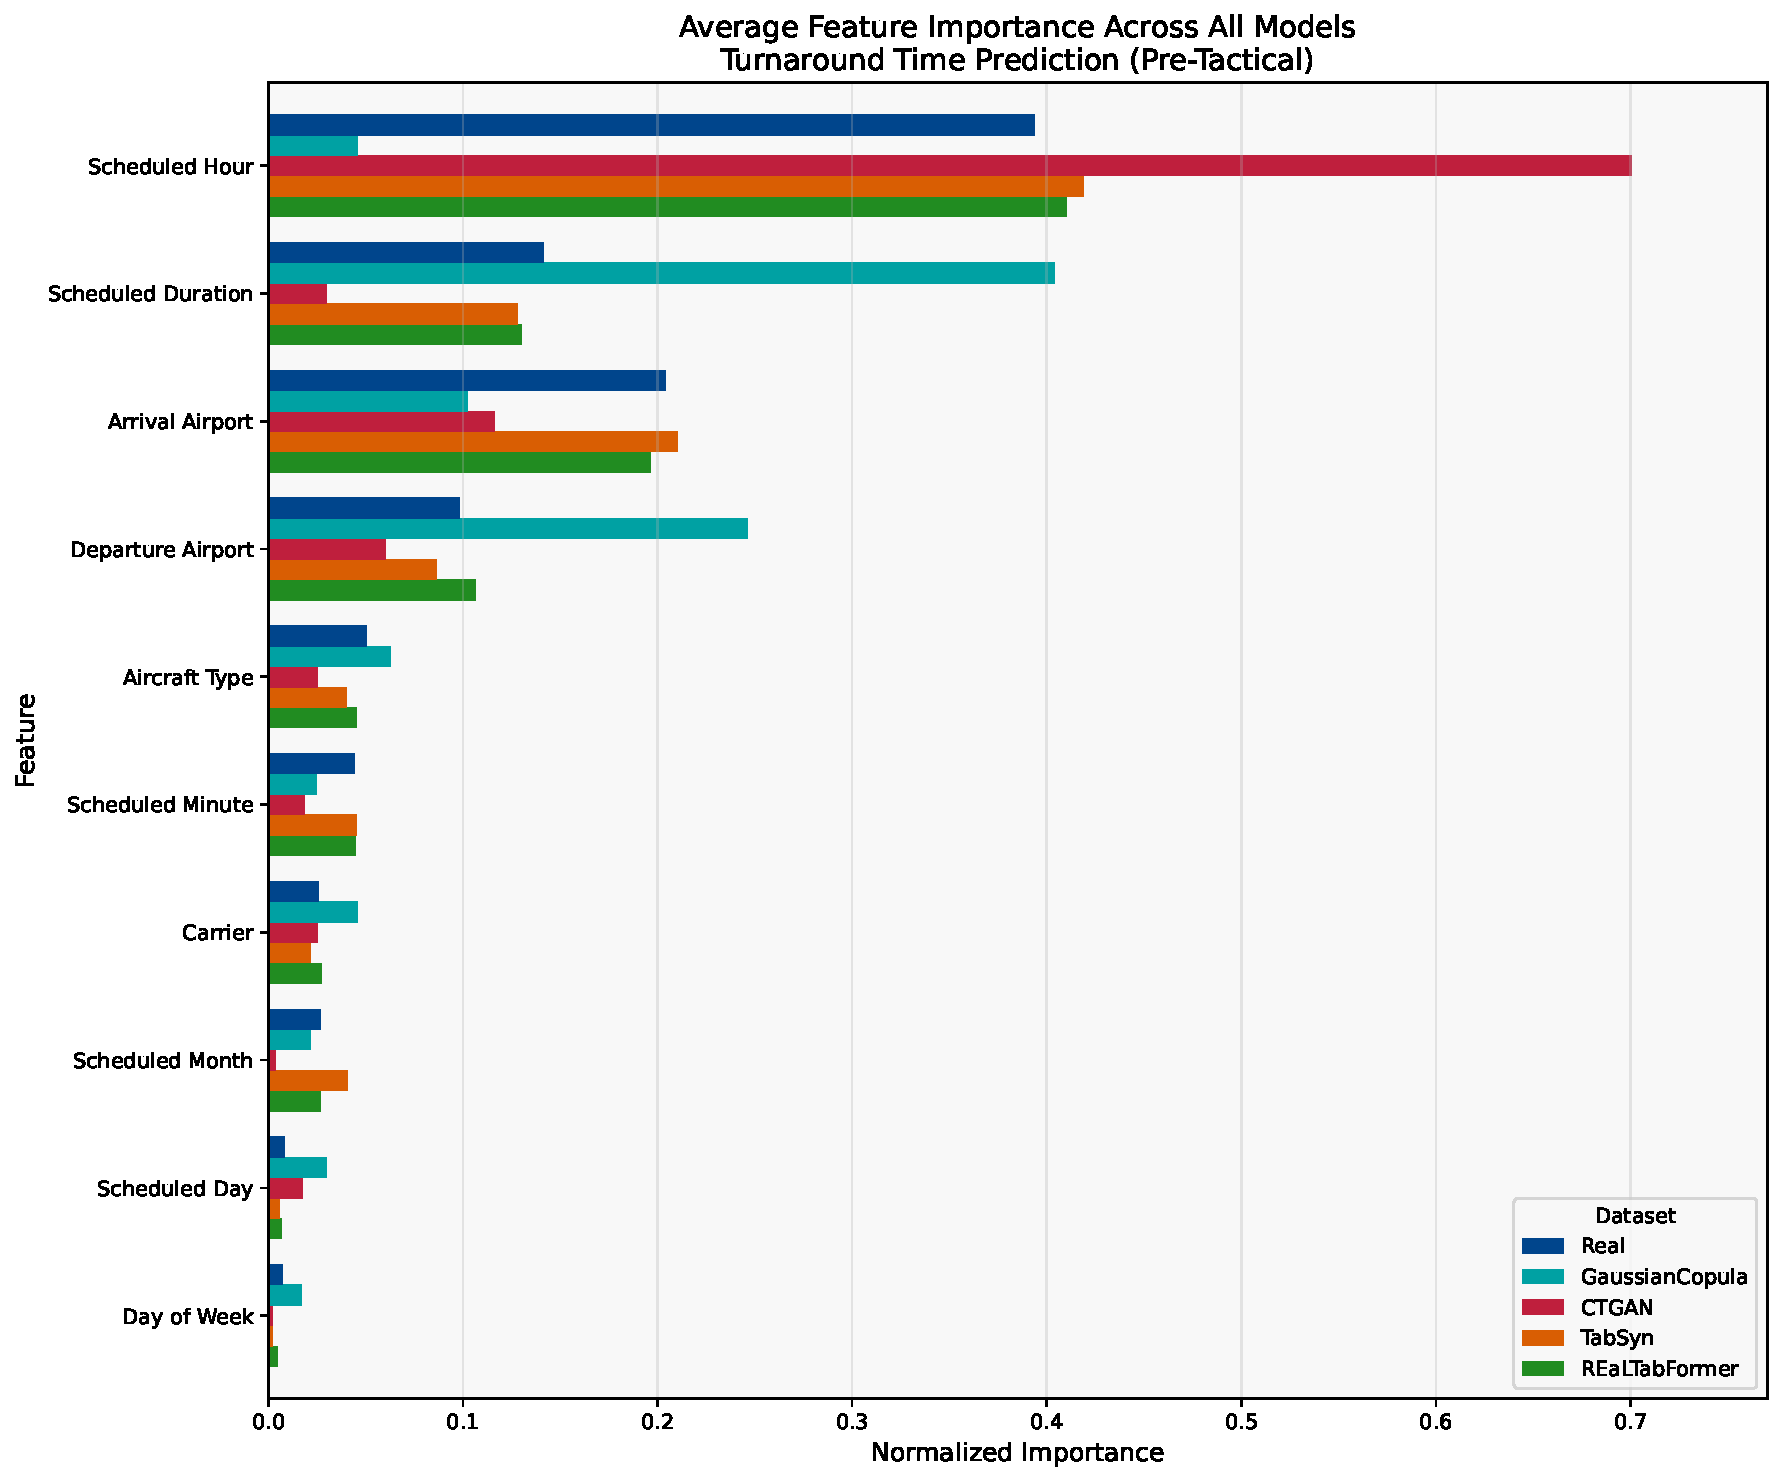
\includegraphics[width=\linewidth]{plots/turnaround_min_pre-tactical/feature_importances/turnaround_min_pre-tactical_all_models_feature_comparison.pdf}
    \caption{Feature importance comparison for pre-tactical turnaround time prediction averaged across all models.}
    \label{fig:turnaround_pre_features}
\end{figure}

The feature importance alignment (Figure~\ref{fig:turnaround_pre_alignment}) shows that  REaLTabFormer and TabSyn achieved perfect alignment scores (1.00), ensuring that models trained on their synthetic data identify precisely the same operational drivers as real-data models. This preservation of causal relationships is crucial for operational applications where understanding which factors drive turnaround variations is as important as prediction accuracy itself.

\begin{figure}[htbp]
    \centering
    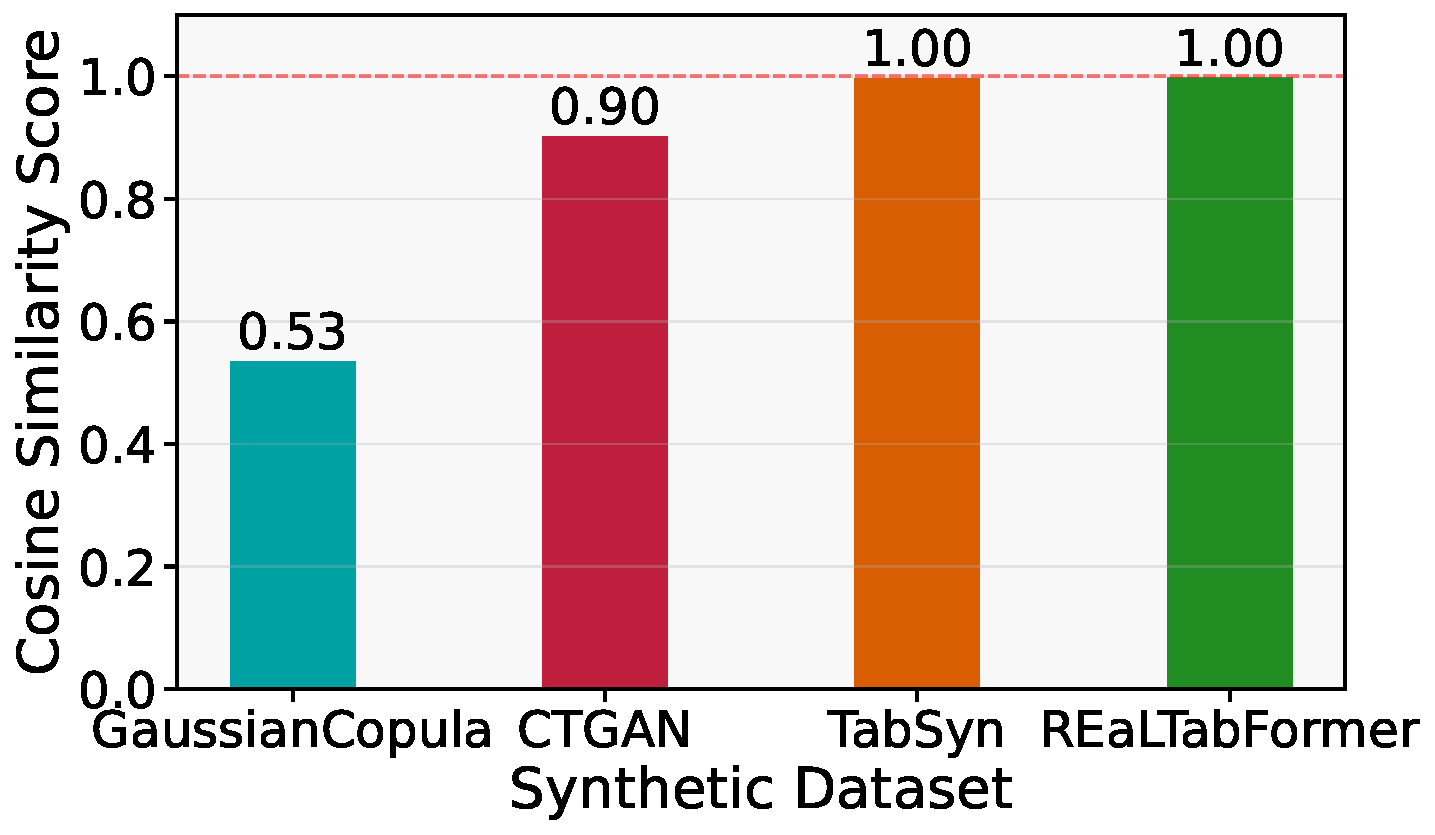
\includegraphics[width=0.8\linewidth]{plots/turnaround_min_pre-tactical/turnaround_min_pre-tactical_avg_alignment_score.pdf}
    \caption{Average feature importance alignment scores for pre-tactical turnaround time prediction.}
    \label{fig:turnaround_pre_alignment}
\end{figure}

\subsection{Cross-Task Performance Analysis}

Analyzing results across all pre-tactical prediction tasks reveals several critical patterns that inform both synthetic data selection and operational expectations:

\textbf{Consistent Generator Hierarchy:} Across all tasks, the performance ranking remained stable: REaLTabFormer (94-97\% utility) $>$ TabSyn (64-93\%) $>$ CTGAN (60-74\%) $>$ Gaussian Copula (55-68\%). This consistency suggests fundamental differences in how each approach captures the complex relationships present in aviation operational data.


\textbf{Feature Relationship Preservation:} Advanced generators (REaLTabFormer, TabSyn) consistently preserved feature importance patterns across all tasks, while simpler methods showed task-dependent degradation. This preservation is crucial for operational deployment, where understanding causal relationships guides resource allocation and process improvement decisions.

\textbf{Fundamental Predictability Limits:} Even with real data, pre-tactical R² values peaked at 0.44 (turnaround), 0.36 (departure delay), and 0.34 (arrival delay). These ceilings reflect inherent uncertainty in aviation operations and should inform realistic expectations for any predictive system, regardless of data source.

\subsection{Operational Implications}

These findings carry significant implications for aviation stakeholders:

\textbf{Strategic Planning Viability:} The high utility scores (94-97\%) achieved by REaLTabFormer indicate that synthetic data can effectively support critical pre-tactical decisions including crew scheduling, gate planning, and resource allocation made hours to days in advance. This capability could democratize advanced analytics across the industry.

\textbf{Research and Development Acceleration:} Preserved feature relationships make synthetic data valuable for algorithm development and benchmarking, allowing researchers to prototype pre-tactical prediction methods without accessing proprietary operational schedules. This could accelerate innovation in aviation analytics.

\textbf{Realistic Expectation Setting:} The modest R² values achieved even with real data highlight inherent uncertainties in pre-tactical prediction. Organizations should design planning processes that accommodate this uncertainty through robust buffers and contingency mechanisms rather than expecting precise predictions.

\textbf{Generator Selection Guidelines:} 
\begin{itemize}
    \item Use REaLTabFormer when prediction accuracy and feature relationship preservation are critical
    \item Consider TabSyn for applications requiring good performance with faster training times
    \item Reserve CTGAN for rapid prototyping scenarios where moderate accuracy loss is acceptable
    \item Limit Gaussian Copula to simple analyses focused primarily on marginal distributions
\end{itemize}





\section{Conclusion}

This study demonstrates that high-quality synthetic flight data can effectively substitute for real operational data in pre-tactical prediction tasks. Advanced generators, particularly REaLTabFormer, achieve 95-97\% of real-data performance while preserving critical feature relationships. However, our results also highlight fundamental predictability limits in pre-tactical scenarios—even with perfect data, uncertainty in flight operations restricts prediction accuracy.
These findings support the operational deployment of synthetic data for strategic planning, research, and algorithm development in aviation. Organizations can leverage synthetic data to develop and validate pre-tactical prediction models without accessing sensitive operational records, democratizing advanced analytics capabilities across the industry. As the aviation industry continues to emphasize data-driven decision-making, high-fidelity synthetic data offers a pathway to broader participation in operational optimization while maintaining commercial confidentiality.


\section*{Acknowledgment}

This paper is based on research conducted within the SynthAIr project, which has received funding from the SESAR Joint Undertaking under the European Union’s Horizon Europe research and innovation program (grant agreement No. 101114847). The views and opinions expressed in this paper are solely those of the authors and do not necessarily reflect those of the European Union or the SESAR 3 Joint Undertaking. Neither the European Union nor the SESAR 3 Joint Undertaking can be held responsible for any use of the information contained herein.


\balance

\bibliographystyle{IEEEtran}
\bibliography{references}




\end{document}
